%% LyX 2.1.3 created this file.  For more info, see http://www.lyx.org/.
%% Do not edit unless you really know what you are doing.
\documentclass{article}\usepackage[]{graphicx}\usepackage[]{color}
%% maxwidth is the original width if it is less than linewidth
%% otherwise use linewidth (to make sure the graphics do not exceed the margin)
\makeatletter
\def\maxwidth{ %
  \ifdim\Gin@nat@width>\linewidth
    \linewidth
  \else
    \Gin@nat@width
  \fi
}
\makeatother

\definecolor{fgcolor}{rgb}{0.345, 0.345, 0.345}
\newcommand{\hlnum}[1]{\textcolor[rgb]{0.686,0.059,0.569}{#1}}%
\newcommand{\hlstr}[1]{\textcolor[rgb]{0.192,0.494,0.8}{#1}}%
\newcommand{\hlcom}[1]{\textcolor[rgb]{0.678,0.584,0.686}{\textit{#1}}}%
\newcommand{\hlopt}[1]{\textcolor[rgb]{0,0,0}{#1}}%
\newcommand{\hlstd}[1]{\textcolor[rgb]{0.345,0.345,0.345}{#1}}%
\newcommand{\hlkwa}[1]{\textcolor[rgb]{0.161,0.373,0.58}{\textbf{#1}}}%
\newcommand{\hlkwb}[1]{\textcolor[rgb]{0.69,0.353,0.396}{#1}}%
\newcommand{\hlkwc}[1]{\textcolor[rgb]{0.333,0.667,0.333}{#1}}%
\newcommand{\hlkwd}[1]{\textcolor[rgb]{0.737,0.353,0.396}{\textbf{#1}}}%

\usepackage{framed}
\makeatletter
\newenvironment{kframe}{%
 \def\at@end@of@kframe{}%
 \ifinner\ifhmode%
  \def\at@end@of@kframe{\end{minipage}}%
  \begin{minipage}{\columnwidth}%
 \fi\fi%
 \def\FrameCommand##1{\hskip\@totalleftmargin \hskip-\fboxsep
 \colorbox{shadecolor}{##1}\hskip-\fboxsep
     % There is no \\@totalrightmargin, so:
     \hskip-\linewidth \hskip-\@totalleftmargin \hskip\columnwidth}%
 \MakeFramed {\advance\hsize-\width
   \@totalleftmargin\z@ \linewidth\hsize
   \@setminipage}}%
 {\par\unskip\endMakeFramed%
 \at@end@of@kframe}
\makeatother

\definecolor{shadecolor}{rgb}{.97, .97, .97}
\definecolor{messagecolor}{rgb}{0, 0, 0}
\definecolor{warningcolor}{rgb}{1, 0, 1}
\definecolor{errorcolor}{rgb}{1, 0, 0}
\newenvironment{knitrout}{}{} % an empty environment to be redefined in TeX

\usepackage{alltt}
\usepackage{ucs}
\usepackage[utf8x]{inputenc}
\usepackage[sc]{mathpazo}
\usepackage[T1]{fontenc}
\usepackage{geometry}

\newenvironment{uzdevums}[1][\unskip]{%
\vspace{3mm}
\noindent
\textbf{#1 uzdevums:}
\noindent}
{}

\geometry{verbose,tmargin=2.5cm,bmargin=2.5cm,lmargin=2.5cm,rmargin=2.5cm}
\setcounter{secnumdepth}{2}
\setcounter{tocdepth}{2}
\usepackage{url}
\usepackage[unicode=true,pdfusetitle,
bookmarks=true,bookmarksnumbered=true,bookmarksopen=true,bookmarksopenlevel=2,
breaklinks=false,pdfborder={0 0 1},backref=false,colorlinks=false]
{hyperref}
\renewcommand{\abstractname}{Anotācija}
\hypersetup{
pdfstartview={XYZ null null 1}}
\IfFileExists{upquote.sty}{\usepackage{upquote}}{}
\begin{document}



\title{41.\ AMO rezultāti tabulās un zīmējumos}

\author{}
\date{}

\maketitle

\begin{abstract}
Šajā dokumentā apkopoti daži 41.\ Atklātās matemātikas olimpiādes (2014.m.g.) rezultātu kop\-sa\-vil\-ku\-mi. Izmantojot izklājlapas, ko publisko LU Neklātienes Matemātikas Skola, aprēķināts dalībnieku skaits, dalības aktivitāte (AMO dalībnieku īpatsvars no visiem attiecīgā vecuma skolēniem), dalība un rezultāti atkarībā no skolēnu \v{g}eogrāfijas, urbanizācijas, valodas, dzimuma. Apkopoti saraksti ar skolotājiem un skolām, kas nodrošinājuši augstu dalību vai ieguvuši lielu punktu kopskaitu. Pārskata nobeigumā minēti dati arī par uzdevumiem --- vidējais punktu skaits un vērtējumu sadalījums, kāda daļa no rēķinātājiem neuzsāka risināt (``mīnusu'' jeb neatrasto risinājumu skaits galavērtējumā), kāda ir konkrētā uzdevuma vērtējumu korelācija ar pārējo uzdevumu vērtējumu summu.
\end{abstract}

\section{Dalībnieku aktivitāte}

Šajā sadaļā atbildēsim uz jautājumu, kāda daļa no 6.klasei atbilstošās vecuma grupas skolēniem piedalījās 41.\ AMO.
Dati par skolēnu skaitu pa re\v{g}ioniem, klasēm un mācību valodām ņemti no IZM publiskotās statistikas --- \url{http://izm.gov.lv/lv/publikacijas-un-statistika/statistika-par-visparejo-izglitibu/2014-2015-m-g}. Dati apkopoti par 9 lielajām pilsētām kā arī par re\v{g}ioniem, kuros nav ietvertas lielās pilsētas. Ar {\em re\v{g}ioniem} domāti NUTS 3 re\v{g}ioni --- sk. \url{http://en.wikipedia.org/wiki/Statistical_regions_of_Latvia} - Kurzeme, Latgale, Pierīga Rīga, Vidzeme, Zemgale.


\subsection{Dalība olimpiādē}



%% col1 = region
%% col2 = participants
%% col3 = total guys
%% col4 = percentage participated

\begin{knitrout}
\definecolor{shadecolor}{rgb}{0.969, 0.969, 0.969}\color{fgcolor}
\begin{tabular}{l|r|r|r}
\hline
  & Participants & All (Grades 5-12) & Activity \%\\
\hline
Liepaja & 48 & 4863 & 0.99\\
\hline
Ventspils & 46 & 2456 & 1.87\\
\hline
Cita Kurzeme & 95 & 9371 & 1.01\\
\hline
Daugavpils & 150 & 5206 & 2.88\\
\hline
Rezekne & 35 & 2453 & 1.43\\
\hline
Cita Latgale & 133 & 10590 & 1.26\\
\hline
Jurmala & 35 & 2507 & 1.40\\
\hline
Cita Pieriga & 376 & 15769 & 2.38\\
\hline
Riga & 1075 & 38631 & 2.78\\
\hline
Valmiera & 95 & 2275 & 4.18\\
\hline
Cita Vidzeme & 272 & 10987 & 2.48\\
\hline
Jekabpils & 44 & 1465 & 3.00\\
\hline
Jelgava & 184 & 3689 & 4.99\\
\hline
Cita Zemgale & 91 & 9739 & 0.93\\
\hline
*** Visa Latvija & 2679 & 120001 & 2.23\\
\hline
\end{tabular}


\end{knitrout}



\begin{knitrout}
\definecolor{shadecolor}{rgb}{0.969, 0.969, 0.969}\color{fgcolor}

{\centering 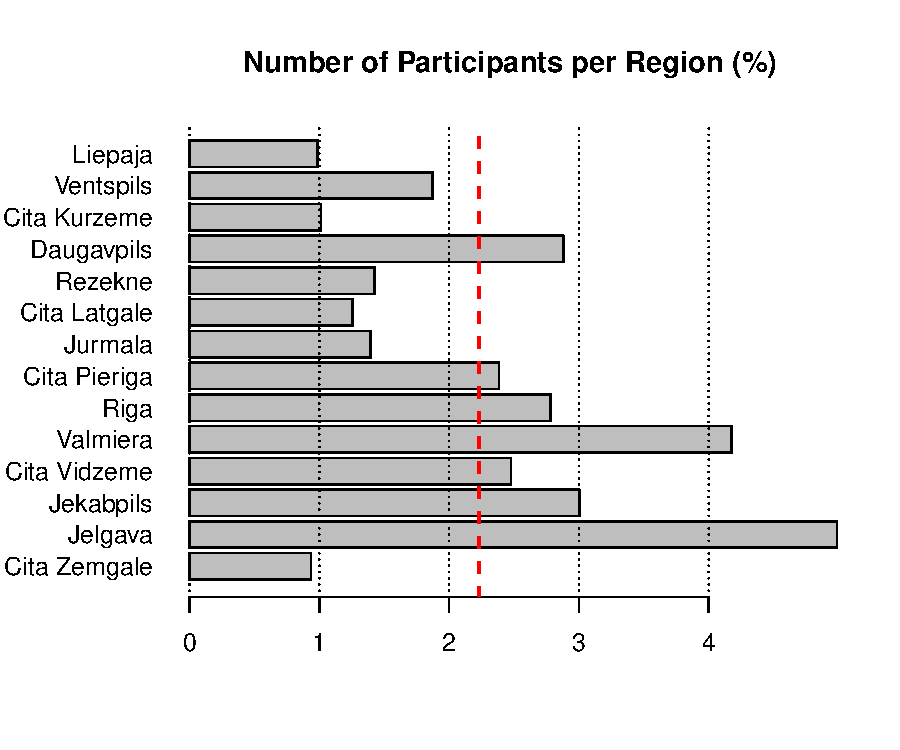
\includegraphics[width=\maxwidth]{figure/minimal-regional-activity-1} 

}



\end{knitrout}


Ir svarīgs ne tikai dalībnieku skaits, bet arī viņu sagatavotības līmenis. Šajā grafikā ikviena olimpiādes dalībnieka rezultātam ir aprēķināta z-normalizētā vērtība jeb {\em z-score}, t.i. no iegūtā punktu skaita jeb {\em raw score} atņem attiecīgās klases aritmētisko vidējo un izdala ar attiecīgās klases standartnovirzi. Pēc tam katrā re\v{g}ionā un katrā klašu grupā atsevišķi rēķina šo z-normalizēto vērtību aritmētisko vidējo. Kā redzams diagrammā, vislabākie vērtējumi olimpiādēs ir Latgalē (zilais grafiks) un Rīgā (sarkanais grafiks). Jaunāko klašu grupās Latgales skolnieku rezultāti pārsniedz valstī vidējo par aptuveni 0.3-0.5 standartnovirzēm. (Tipiski jebkurā klašu grupā punktu skaita standartnovirze ir $\sigma \in [8,11]$, t.i. Latgales skolēnu rezultāti vidēji ir par 3-4 punktiem augstāki nekā citur. Tomēr salīdzināt iegūto punktu starpības nav visai korekti, jo katrā olimpiādes gadā un klašu grupā uzdevumu grūtība un tātad arī punktu izkliede var jūtami atšķirties.)


\begin{knitrout}
\definecolor{shadecolor}{rgb}{0.969, 0.969, 0.969}\color{fgcolor}

{\centering 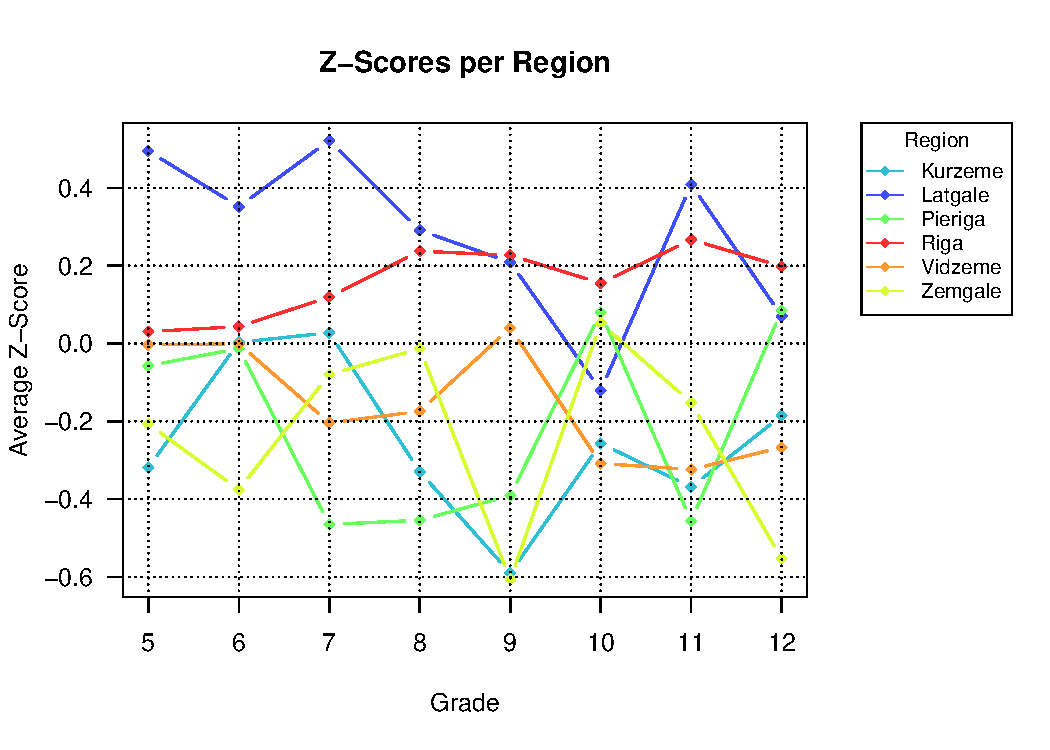
\includegraphics[width=\maxwidth]{figure/minimal-averages-per-region-1} 

}



\end{knitrout}



% 1+9+5 aktivitāšu skaitļi pa reģioniem
% Katram no 15 reģioniem dota dzimumu proporcija
%% Stabiņi grupās pa 3 - visi/meitenes/zēni.

% 1+9+5 aktivitāšu skaitļi pa reģioniem - darbi latviešu valodā
% Katram no 15 reģioniem dota dzimumu proporcija

% 1+9+5 aktivitāšu skaitļi pa reģioniem - darbi krievu valodā
% Katram no 15 reģioniem dota dzimumu proporcija

\begin{knitrout}
\definecolor{shadecolor}{rgb}{0.969, 0.969, 0.969}\color{fgcolor}

{\centering 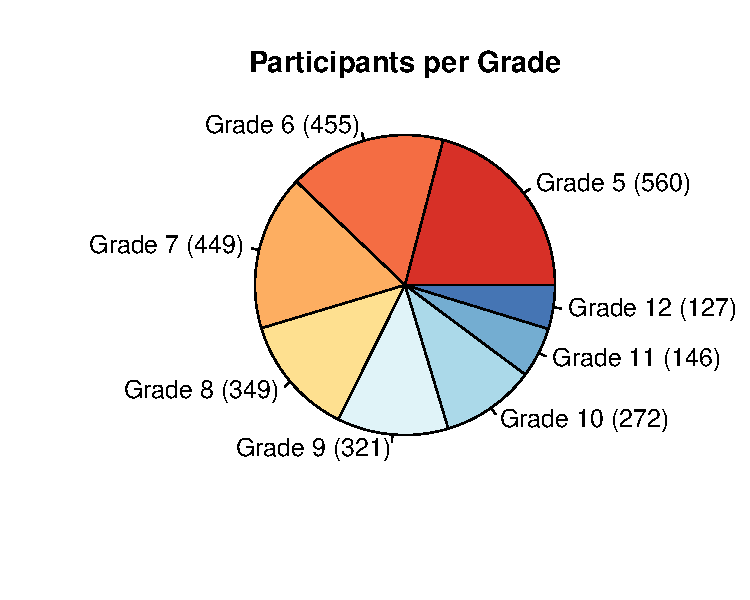
\includegraphics[width=\maxwidth]{figure/minimal-per-class-1} 

}



\end{knitrout}

\subsection{Dalība un sociāli-ekonomiskie rādītāji}

% Trīs 14-bumbulīšu diagrammas

Šeit varētu ievietot diagrammas pa novadiem vai novadu grupām, kas parāda divu parametru attiecību (varētu būt runa par burbulīšu diagrammām, ko zīmē divās dimensijās; turklāt burbulīša laukums ir aptuveni proporcionāls skolēnu skaitam olimpiādē).

\begin{itemize}
\item Sociāli-ekonomisko rādītāju --- bezdarbu, IIN uz 1 iedzīvotāju, pašvaldības izdevumus uz 1 skolēnu vai skolēnu skaitu skolā.
\item Dalībnieku aktivitāti (dalībnieku attiecību pret visiem skolēniem novadā) kā arī olimpiādes summāro rezultātu (punktu summas attiecību pret visiem skolēniem novadā).
\end{itemize}

Šādas diagrammas palīdzētu saprast, kādi sociālie priekšnoteikumi veicina interesi par olimpiādēm, kāda izglītības politika (piemēram, mazo skolu saglabāšana vai slēgšana; lielāki vai mazāki izdevumi par vienu skolēnu) varētu pozitīvi iespaidot olimpiāžu rezultātus.

\subsection{Dalībnieku struktūra}



%% Segmenti -- 6 NUTS reģioni
% http://en.wikipedia.org/wiki/Statistical_regions_of_Latvia

Atklātajā matemātikas olimpiādē sastopami darbi latviešu un krievu valodās. Valodu būtu visprecīzāk noteikt, aplūkojot katru konkrēto darbu. Par 41.\ AMO mums šādas informācijas nav, tādēļ valodu secinājām no skolēna re\v{g}istrācijā minētās informācijas, vai arī viņa skolā dominējošo valodu, bet jauktām skolām --- valodu, kas visbiežāk sastopama pieteiktā matemātikas skolotāja audzēkņu vidū. Katras klases joslas iekšpusē iezīmēts balts aplītis, kurš parāda latviešu skolēnu īpatsvaru visu attiecīgās klases audzēkņu vidū. Visām klašu grupām, izņemot 5.\ klasi, latviešu darbu īpatsvars 41.\ AMO ir nedaudz lielāks nekā skolēnu īpatsvars latviešu plūsmas skolās kopumā. Krievu valodā rakstošie skolēni olimpiādē piedalās nedaudz retāk, toties viņu rezultāti mēdz būt labāki (sk. apakšnodaļu "Pirmie 100 skolotāji pēc dalībnieku skaita augšējā kvartilē").

Kā redzams, dalība AMO nav pilnīgi proporcionāla latviešu un krievu skolu audzēkņu vidū. Tomēr atšķirības nav lielas --- pie pašreizējās olimpiādes apmeklētības, šo statistiku varētu jūtami izmainīt, papildus piesaistot dalībai olimpiādē dažus desmitus skolēnu. Latvijas vispārizglītojošajās skolās mācības mēdz notikt arī poļu, ukraiņu, baltkrievu, angļu un franču valodās. Šo skolu audzēkņi var izvēlēties rakstīt darbu latviski vai krieviski. Viņu darbi pieskaitīti atkarībā no re\v{g}istrācijā norādītās valodas.


%% K/L skaita attiecība pa klasēm
\begin{knitrout}
\definecolor{shadecolor}{rgb}{0.969, 0.969, 0.969}\color{fgcolor}

{\centering 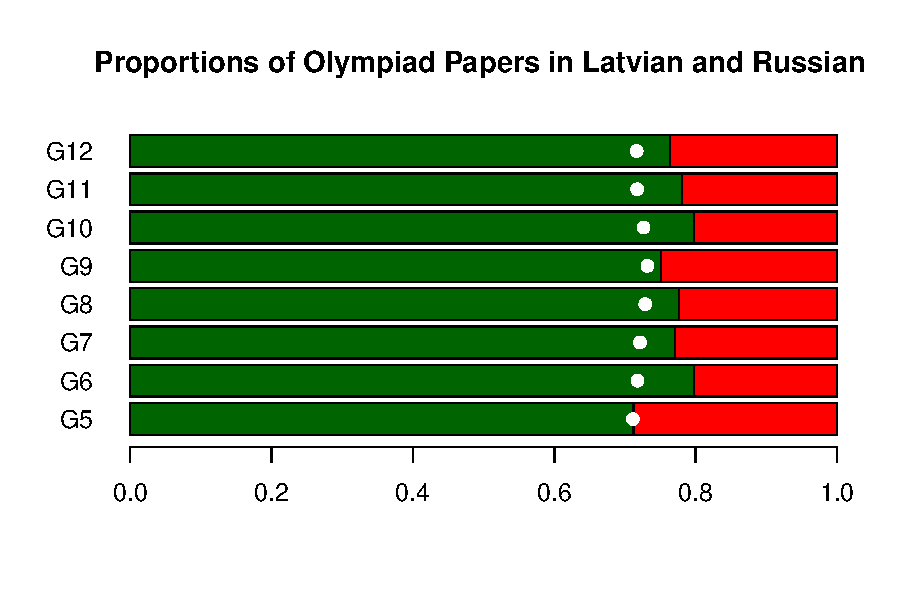
\includegraphics[width=\maxwidth]{figure/minimal-lang-proportions-1} 

}



\end{knitrout}



%% Marimekko diagrammas - dalībnieku dzimumu struktūra pa reģioniem.
% https://learnr.wordpress.com/2009/03/29/ggplot2_marimekko_mosaic_chart/
%% Segmenti -- 4 urbanizācijas tipi (LV-meitenes, LV-zēni, RU-meitenes, RU-zēni)

Dalībnieku demogrāfisko struktūru var attēlot arī dažādām parametru kombinācijām. Šajā zīmējumā redzams dalībnieku sadalījums pa klasēm (vertikālie stabiņi), un katras klases iekšienē --- arī pa darbu valodām un dalībnieku dzimumiem. Skolēna dzimums re\v{g}istrācijas un rezultātu datos nav dots, 41.\ AMO tos noteicām pēc skolēna vārda. Pasaulē ir matemātikas sacensības, piemēram, EGMO (European Girls' Mathematical Olympiad), kuru nolūks ir veicināt meiteņu pievēršanos eksaktajām un inženierzinātnēm. Kopš olimpiādes pirmsākumiem (2012.\ gadā Kembridžā) EGMO piedalās arī četras vecāko klašu skolnieces no Latvijas. Sk. \url{https://www.egmo.org/}.

Latviešu valodā rakstītajiem darbiem zēnu un meiteņu ir aptuveni vienāds skaits, bet krievu valodā rakstītajiem darbiem meiteņu vecāko klašu grupās ir pat divreiz mazāk nekā zēnu.

\begin{knitrout}
\definecolor{shadecolor}{rgb}{0.969, 0.969, 0.969}\color{fgcolor}\begin{kframe}


{\ttfamily\noindent\itshape\color{messagecolor}{\#\# Loading required package: ggplot2}}

{\ttfamily\noindent\color{warningcolor}{\#\# Warning: package 'ggplot2' was built under R version 3.2.4}}\end{kframe}

{\centering 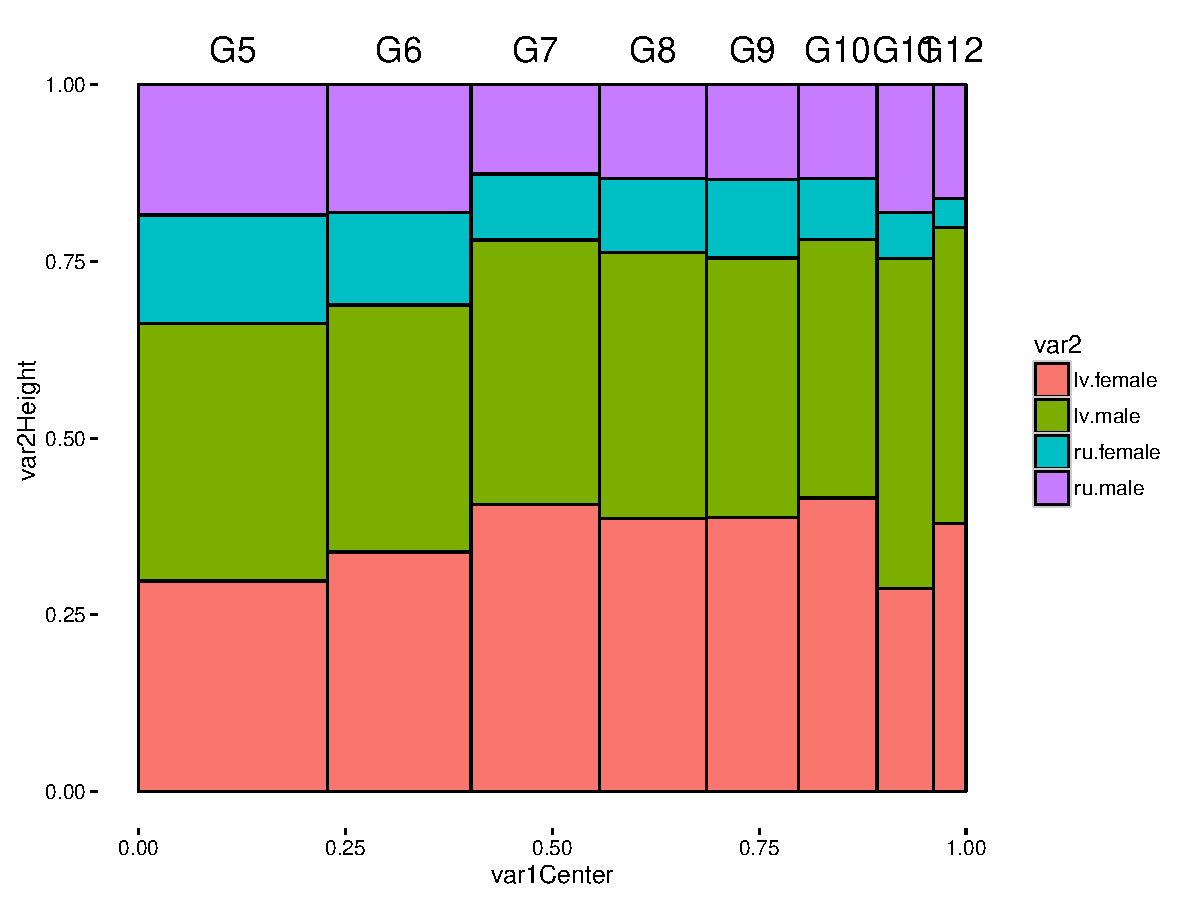
\includegraphics[width=\maxwidth]{figure/minimal-demography-segments-1} 

}



\end{knitrout}



%%<<demography-segments, echo=FALSE, fig.width=7, fig.height=6>>=
% options(warn=-1)
% library(reshape)
% library(ggplot2)
%
% results <- getExtResults(41)
% pupilsPerGrade <- as.vector(table(results$Grade))
% pupilsPerGradePercent <- 100*pupilsPerGrade/sum(pupilsPerGrade)
%
% AlphaVals <- 100*as.vector(table(results$Grade[
%   results$Dzimums=="Male" & results$Language=="L"]))/pupilsPerGrade
% BetaVals <- 100*as.vector(table(results$Grade[
%   results$Dzimums=="Female" & results$Language=="L"]))/pupilsPerGrade
% GammaVals <- 100*as.vector(table(results$Grade[
%   results$Dzimums=="Male" & results$Language=="K"]))/pupilsPerGrade
% DeltaVals <- 100*as.vector(table(results$Grade[
%   results$Dzimums=="Female" & results$Language=="K"]))/pupilsPerGrade
%
%
% df <- data.frame(
%   segment = 5:12,
%   segpct = pupilsPerGradePercent,
%   lv.males = AlphaVals,
%   lv.females = BetaVals,
%   ru.males = GammaVals,
%   ru.females = DeltaVals)
%
% df$xmax <- cumsum(df$segpct)
% df$xmin <- df$xmax - df$segpct
% df$segpct <- NULL
%
% dfm <- melt(df, id = c("segment", "xmin", "xmax"))
%
% dfm1 <- ddply(dfm, .(segment), transform, ymax = cumsum(value))
% dfm1 <- ddply(dfm1, .(segment), transform,
%               ymin = ymax - value)
%
%
% dfm1$xtext <- with(dfm1, xmin + (xmax - xmin)/2)
% dfm1$ytext <- with(dfm1, ymin + (ymax - ymin)/2)
%
% p <- ggplot(dfm1, aes(ymin = ymin, ymax = ymax,
%                       xmin = xmin, xmax = xmax, fill = variable))
%
% p1 <- p + geom_rect(colour = I("grey"))
%
% p2 <- p1 + geom_text(
%   aes(x = xtext, y = ytext,
%       label = ifelse(segment == "A",
%                      paste(variable," - ", value, "%", sep = ""),
%                      sprintf("%2.1f%%", value))),
%   size = 3.5)
%
%
%
% p3 <- p2 + geom_text(aes(x = xtext, y = 103,
%                          label = sprintf("G%d", segment)), size = 4)
%
%
% p3 + theme_bw() +
%   labs(x = NULL, y = NULL,fill = NULL) +
%   scale_fill_brewer(palette = "Set2") +
%   theme(legend.position = "bottom",
%        panel.grid.major = element_line(colour = NA),
%        panel.grid.minor = element_line(colour = NA))
% options(warn=0)
%%@

\subsection{Dalībnieku valodas lielajās pilsētās}

Šajā diagrammā mazie aplīši parāda olimpiādes darbu valodu proporciju Latvijas lielākajās pilsētās (9 lielās pilsētas kā arī Ogre, Tukums un Cēsis, kurās iedzīvotāju skaits ir tuvu 20 tūkstošiem - t.i. daudz neatšķiras no Valmieras un Jēkabpils iedzīvotāju skaita). Aplīša laukums ir aptuveni proporcionāls dalībnieku skaitam no attiecīgās pilsētas.

\begin{knitrout}
\definecolor{shadecolor}{rgb}{0.969, 0.969, 0.969}\color{fgcolor}\begin{kframe}


{\ttfamily\noindent\color{warningcolor}{\#\# Warning: package 'classInt' was built under R version 3.2.5}}

{\ttfamily\noindent\color{warningcolor}{\#\# Warning: package 'gridBase' was built under R version 3.2.5}}

{\ttfamily\noindent\color{warningcolor}{\#\# Warning: package 'maptools' was built under R version 3.2.5}}

{\ttfamily\noindent\itshape\color{messagecolor}{\#\# Loading required package: sp}}

{\ttfamily\noindent\color{warningcolor}{\#\# Warning: package 'sp' was built under R version 3.2.5}}

{\ttfamily\noindent\itshape\color{messagecolor}{\#\# Checking rgeos availability: FALSE\\\#\#\ \ 	Note: when rgeos is not available, polygon geometry 	computations in maptools depend on gpclib,\\\#\#\ \ 	which has a restricted licence. It is disabled by default;\\\#\#\ \ 	to enable gpclib, type gpclibPermit()}}

{\ttfamily\noindent\itshape\color{messagecolor}{\#\# Loading required package: bitops}}\end{kframe}

{\centering 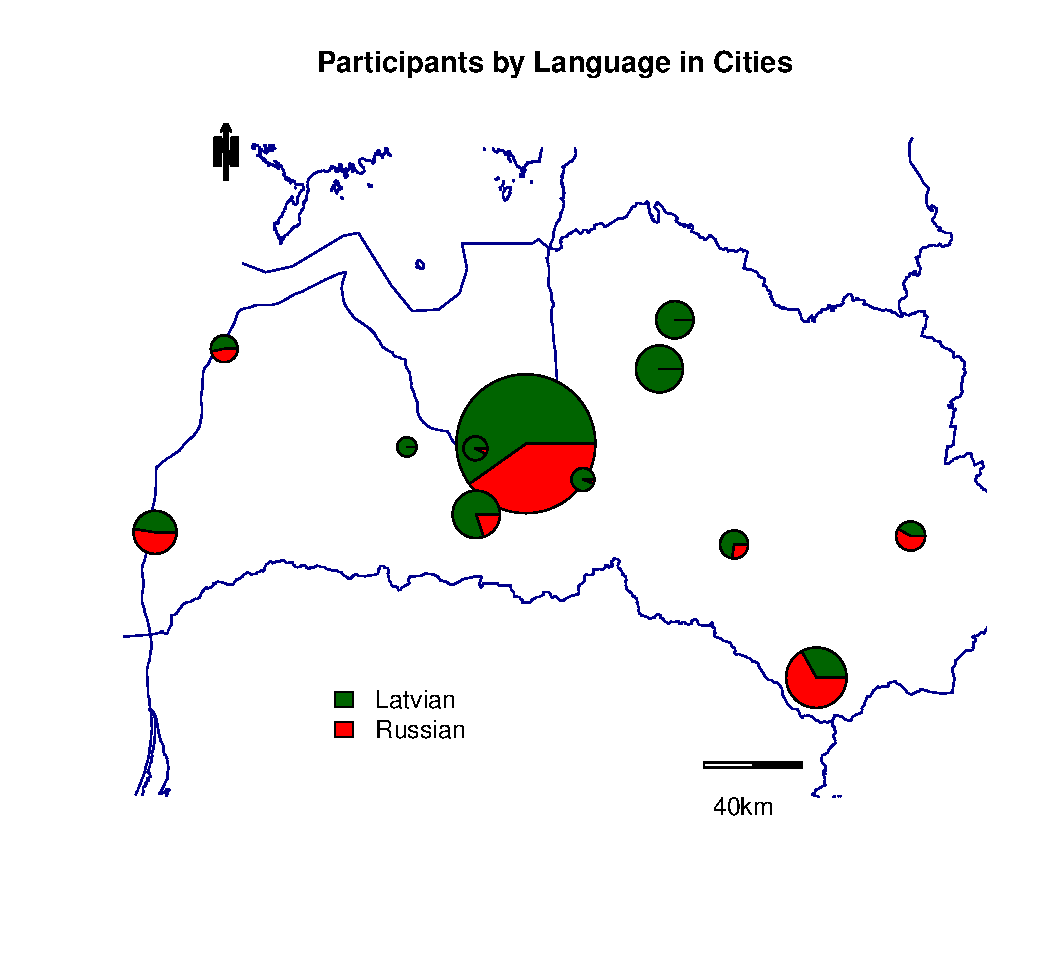
\includegraphics[width=\maxwidth]{figure/minimal-language-per-city-1} 

}



\end{knitrout}





\section{Vidējie rezultāti dalībnieku kategorijām}

Zīmējumā dots rezultātu intervāls katrai klasei. ``Kastītes'' kreisā mala atbilst apakšējai kvartilei, labā mala --- augšējai kvartilei, bet platā zilā svītriņa vidū --- mediānai. Ja klases darbus sakārtotu punktu pieaugšanas secībā un sadalītu četrās vienādās daļās, tad viszemāko punktu ieguvēju ceturtdaļa atrastos uz kreisās ūsas, divas vidējās ceturtdaļas --- kastītes iekšpusē, bet augšējā ceturtdaļa --- uz labās ūsas. Kā redzams attēlā, 12.\ klases skolnieku iegūtais punktu skaits ir būtiski lielāks nekā citu klašu risinātājiem. To varētu izskaidrot daži viegli uzdevumi, kuri ir 12.\ klases komplektā.

\begin{knitrout}
\definecolor{shadecolor}{rgb}{0.969, 0.969, 0.969}\color{fgcolor}

{\centering 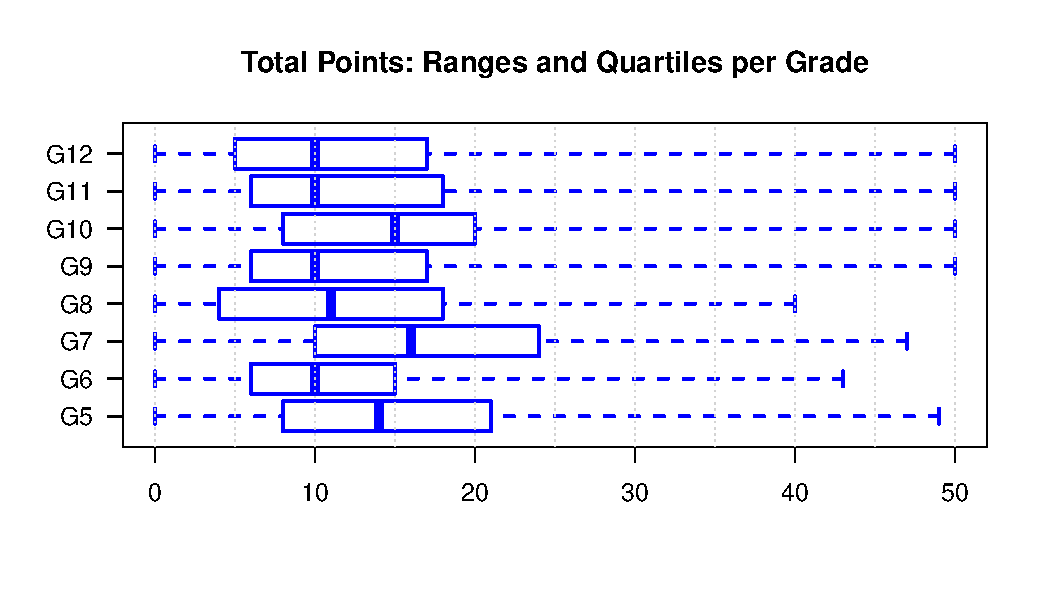
\includegraphics[width=\maxwidth]{figure/minimal-boxplots-per-grade-1} 

}



\end{knitrout}




%% Visu dalībnieku darbi, iekrāsotas godalgotās vietas
%% Meiteņu un zēnu darbi (Meitenes zīmējam tanī pašā histogrammā)
%% Meitenes ir sazīmētas apakšā.

%% Urbaniz. tips. Rīgas, 8 lielo pilsētu, mazpilsētu un lauku darbi

%% Latviešu un krievu valodā rakstītie darbi

%% Latviešu un krievu valodā rakstītie darbi -- tikai 9 lielajās pilsētās


\section{Skolas un skolotāji}



Tabulā apkopoti dati par matemātikas skolotājiem:

\noindent
{\bf Participants} --- Cik dalībnieku piedalījās olimpiādē.\\
{\bf Q3} --- Cik no viņiem ir ieguvuši rezultātu savas klases augšējā kvartilē. Punktu skaits, kas nepieciešams iekļūšanai augšējā kvartilē, ir atkarīgs no klases ($Q_3(Grade5)=21\;$, $Q_3(Grade6)=15\;$, $Q_3(Grade7)=24\;$, $Q_3(Grade8)=18\;$, $Q_3(Grade9)=17\;$, $Q_3(Grade10)=20\;$, $Q_3(Grade11)=18\;$, $Q_3(Grade12)=17\;$.)\\
{\bf Points} --- Kāda ir attiecīgā skolotāja sagatavoto skolēnu punktu summa.\\
{\bf School} --- Skolotāja pārstāvētā skola.



Tajos gadījumos, kad skolēns norādījis vairākus skolotājus, attiecīgo dalībnieku un viņa punktus pieskaita visiem skolotājiem. Kā redzams tabuliņā, vairums risinātāju (93.3\%) norādījuši tieši vienu skolotāju.


\begin{knitrout}
\definecolor{shadecolor}{rgb}{0.969, 0.969, 0.969}\color{fgcolor}
\begin{tabular}{l|r}
\hline
Noraditi skolotaji & Darbu skaits\\
\hline
0 & 34\\
\hline
1 & 2953\\
\hline
2 & 157\\
\hline
3 & 20\\
\hline
Kopa & 3164\\
\hline
\end{tabular}


\end{knitrout}





Turpmākajās tabulās doti trīs dažādu veidu reitingi --- pirmie 100 skolotāji (pavisam bija 735 skolotāju, kuru vārdus skolēni norādīja savos darbos). Pirmajā reitingā skolotāji sakārtoti atbilstoši kopīgajam dalībnieku skaitam; otrajā reitingā --- atbilstoši dalībnieku skaitam, kuru rezultāts ir augšējā kvartilē, trešajā reitingā --- atbilstoši visu dalībnieku kopīgajam punktu skaitam. Šajos reitingos var ievērot, ka masveidīgākā dalība olimpiādēs ir skolēniem no Rīgas 1.\ \v{g}imnāzijas, savukārt pēc potenciālo laureātu un punktu skaita priekšgalā izvirzās Daugavpils Krievu vidusskola-licejs.

{\em Apzināti neveidojām reitingu pēc ``aritmētiskā vidējā rezultāta'', jo arī neliela punktu skaita saņemšana olimpiādē ir pozitīvs sasniegums; nebūtu attaisnojami tādi reitingi, kuros masveidīgāka dalība vilktu skolas vai skolotāja kopvērtējumu lejup.}


% Skolas pēc dalībnieku skaita

% Skolas pēc savāktajiem punktiem

%% Skolotāji pēc dalībnieku skaita

\newpage
{\bf Pirmie 100 skolotāji pēc dalībnieku skaita}\\ \nopagebreak
\begin{knitrout}
\definecolor{shadecolor}{rgb}{0.969, 0.969, 0.969}\color{fgcolor}
\begin{tabular}{r|l|r|r|r|l}
\hline
Num & Name & Participants & Q3 & Points & School\\
\hline
1 & Dace Andzane & 48 & 26 & 1217 & Rigas Valsts 1. gimnazija\\
\hline
2 & Dzintars Zicans & 45 & 14 & 792 & Rigas Valsts 1. gimnazija\\
\hline
3 & Inese Lagzda & 43 & 26 & 848 & Rigas Valsts 1. gimnazija\\
\hline
4 & Irena Oksenuka & 30 & 16 & 519 & Daugavpils Krievu vidusskola - licejs\\
\hline
5 & Daiga Jekabsone & 29 & 9 & 457 & Siguldas Valsts gimnazija\\
\hline
6 & Ingrida Veilande & 27 & 4 & 317 & Adazu vidusskola\\
\hline
7 & Inese Lude & 25 & 3 & 265 & Andreja Pumpura Rigas 11. pamatskola\\
\hline
8 & Agrita Bartusevica & 24 & 4 & 324 & Cesu Valsts gimnazija\\
\hline
9 & Emils Veide & 23 & 12 & 568 & Rigas Valsts 1. gimnazija\\
\hline
10 & Anita Slaidina & 23 & 12 & 513 & Cesu Valsts gimnazija\\
\hline
11 & Inga Ruskule & 23 & 4 & 256 & Priekulu vidusskola\\
\hline
12 & Alina Magomedova & 22 & 11 & 391 & Daugavpils Krievu vidusskola - licejs\\
\hline
13 & Aija Vasilevska & 21 & 11 & 404 & Rigas Valsts 1. gimnazija\\
\hline
14 & Zane Kaibe & 21 & 8 & 408 & Rigas 64.vidusskola\\
\hline
15 & Nina Juste & 20 & 9 & 342 & Agenskalna Valsts gimnazija\\
\hline
16 & Laila Aigare & 19 & 9 & 271 & Rigas Valda Zalisa sakumskola\\
\hline
17 & Margita Jirgensone & 19 & 5 & 200 & Jelgavas Spidolas gimnazija\\
\hline
18 & Vera Solovjova & 18 & 7 & 255 & Rigas 10.vidusskola\\
\hline
19 & Karmena Liepina & 18 & 6 & 268 & Rigas Valsts 1. gimnazija\\
\hline
20 & Valentina Cesnokova & 18 & 4 & 227 & Rigas 13.vidusskola\\
\hline
21 & Alesja Sapkova & 17 & 12 & 357 & Daugavpils Saskanas pamatskola\\
\hline
22 & Anita Indare & 17 & 4 & 212 & Jelgavas Spidolas gimnazija\\
\hline
23 & Irina Morusa & 17 & 2 & 219 & Rigas 72. vidusskola\\
\hline
24 & Ludmila Ulinska & 16 & 9 & 352 & Daugavpils Saskanas pamatskola\\
\hline
25 & Natalja Mosolova & 16 & 4 & 209 & Rigas 13.vidusskola\\
\hline
26 & Daina Brinke & 16 & 0 & 173 & Rigas Valsts 2. gimnazija\\
\hline
27 & Inta Ozolina & 15 & 5 & 242 & Siguldas pilsetas vidusskola\\
\hline
28 & Liene Cerpa & 15 & 4 & 187 & Siguldas pilsetas vidusskola\\
\hline
29 & Lidija Lisovska & 15 & 2 & 195 & Cesu pilsetas pamatskola\\
\hline
30 & Inga Kauskale & 15 & 1 & 121 & Mezciema pamatskola\\
\hline
31 & Irina Polakova & 14 & 10 & 334 & Daugavpils Krievu vidusskola - licejs\\
\hline
32 & Stanislav Didych & 14 & 9 & 322 & Daugavpils Krievu vidusskola - licejs\\
\hline
33 & Olga Sheremet & 14 & 6 & 241 & Rigas Zolitudes gimnazija\\
\hline
34 & Inga Neilande & 14 & 2 & 160 & Jelgavas 4.sakumskola\\
\hline
35 & Olga Kostenko & 14 & 2 & 160 & Rigas Rinuzu vidusskola\\
\hline
36 & Inese Boze & 14 & 1 & 151 & Draudziga Aicinajuma Cesu Valsts gimnazija\\
\hline
37 & Inna Glebova & 13 & 7 & 243 & Rigas 34. vidusskola\\
\hline
38 & Indra Upite-Dambite & 13 & 6 & 279 & Siguldas Valsts gimnazija\\
\hline
39 & Lilija Roldugina & 13 & 5 & 205 & Rigas 40. vidusskola\\
\hline
40 & Viola Levina & 13 & 1 & 168 & Valkas gimnazija\\
\hline
41 & Jolanta Klamere & 13 & 1 & 109 & J. Cakstes Liepajas pilsetas 10. vidusskola\\
\hline
42 & Regina Simanovska & 12 & 7 & 268 & Rigas Valsts 1. gimnazija\\
\hline
43 & Nadezda Koleda & 12 & 6 & 221 & Rigas 34. vidusskola\\
\hline
44 & Liene Andzane & 12 & 1 & 119 & Kraslavas Valsts gimnazija\\
\hline
45 & Iveta Perkona & 12 & 0 & 119 & Jelgavas 3.sakumskola\\
\hline
46 & Anna Jansone & 11 & 7 & 272 & Rigas Valsts 1. gimnazija\\
\hline
47 & Ilze Vitina & 11 & 1 & 153 & Sakumskola "Taurenitis"\\
\hline
48 & Ira Nikiforova & 11 & 1 & 79 & Plavinu novada gimnazija\\
\hline
49 & Vaira Buza & 11 & 0 & 112 & Draudziga Aicinajuma Cesu Valsts gimnazija\\
\hline
50 & Dagnija Kikane & 11 & 0 & 94 & Adazu vidusskola\\
\hline
\end{tabular}


\end{knitrout}


\begin{knitrout}
\definecolor{shadecolor}{rgb}{0.969, 0.969, 0.969}\color{fgcolor}
\begin{tabular}{r|l|r|r|r|l}
\hline
Num & Name & Participants & Q3 & Points & School\\
\hline
51 & Svetlana Elksnina & 11 & 0 & 68 & Daugavpils Krievu vidusskola - licejs\\
\hline
52 & Dina Vertasonoka & 11 & 0 & 61 & Daugavpils 15.vidusskola\\
\hline
53 & Nadezda Zuka & 11 & 0 & 60 & Rigas 21.vidusskola\\
\hline
54 & Rita Hrapane & 10 & 9 & 218 & Daugavpils Krievu vidusskola - licejs\\
\hline
55 & Ingrida Brizga & 10 & 6 & 176 & Cesu 2. pamatskola\\
\hline
56 & Tamara Jersova & 10 & 4 & 175 & Rigas 10.vidusskola\\
\hline
57 & Dace Celina & 10 & 4 & 154 & Agenskalna sakumskola\\
\hline
58 & Evija Slokenberga & 10 & 3 & 185 & Jelgavas Valsts gimnazija\\
\hline
59 & Edite Teterovska & 10 & 3 & 157 & Rigas Lietuviesu vidusskola\\
\hline
60 & Laila Ruke & 10 & 3 & 154 & Cesu Valsts gimnazija\\
\hline
61 & Zane Berga & 10 & 3 & 140 & Straupes pamatskola\\
\hline
62 & Ligita Neimane & 10 & 2 & 148 & Cesu pilsetas pamatskola\\
\hline
63 & Aleksandra Fjodorova & 10 & 2 & 97 & Rigas Centra humanitara vidusskola\\
\hline
64 & Eva Jakobsone & 10 & 1 & 121 & Adazu vidusskola\\
\hline
65 & Valda Bickova & 10 & 1 & 121 & Uzvaras vidusskola\\
\hline
66 & Zinaida Panarada & 10 & 1 & 102 & Jelgavas 6.vidusskola\\
\hline
67 & Aivars Ancupans & 10 & 1 & 90 & Agenskalna Valsts gimnazija\\
\hline
68 & Liga Plauca & 10 & 0 & 103 & Agenskalna Valsts gimnazija\\
\hline
69 & Irina Macanova & 10 & 0 & 95 & Olaines 2.vidusskola\\
\hline
70 & Nadezda Leitane & 10 & 0 & 75 & Valmieras Valsts gimnazija\\
\hline
71 & Selga Lukjanska & 10 & 0 & 74 & Cesu 1. pamatskola\\
\hline
72 & Valda Zviedre & 10 & 0 & 20 & Malpils novada vidusskola\\
\hline
73 & Iveta Zarane & 9 & 7 & 230 & Daugavpils Krievu vidusskola - licejs\\
\hline
74 & Irena Kozlovska & 9 & 4 & 158 & Puskina  licejs\\
\hline
75 & Veneranda Springe & 9 & 4 & 135 & Rudzatu vidusskola\\
\hline
76 & Olga Malkova & 9 & 3 & 145 & Liepajas A.Puskina 2.vidusskola\\
\hline
77 & Aiva Rituma & 9 & 3 & 138 & Dobeles Valsts gimnazija\\
\hline
78 & Kaiva Treija & 9 & 3 & 115 & Rigas Valsts 2. gimnazija\\
\hline
79 & Anna Gustava & 9 & 2 & 124 & Rigas 25.vidusskola\\
\hline
80 & Kristine Gaigala & 9 & 2 & 90 & Rigas 64.vidusskola\\
\hline
81 & Laura Freija & 9 & 1 & 125 & Rigas Valsts 2. gimnazija\\
\hline
82 & Laila Berzina & 9 & 1 & 91 & Priekulu vidusskola\\
\hline
83 & Agita Seglicka & 9 & 1 & 79 & Vecumnieku vidusskola\\
\hline
84 & Inara Veita & 9 & 0 & 114 & Valmieras Pargaujas gimnazija\\
\hline
85 & Aleksandra Ivanova & 9 & 0 & 81 & Zvejniekciema vidusskola\\
\hline
86 & Anete Zaca & 9 & 0 & 66 & Jelgavas Valsts gimnazija\\
\hline
87 & Antra Punovska & 9 & 0 & 59 & Andreja Eglisa Laudonas vidusskola\\
\hline
88 & Dzintra Zingule & 9 & 0 & 55 & Jelgavas 3.sakumskola\\
\hline
89 & Ilze Kale & 9 & 0 & 47 & Grobinas gimnazija\\
\hline
90 & Mara Ieleja & 9 & 0 & 44 & Limbazu 3. vidusskola\\
\hline
91 & Gunta Kuzmina & 9 & 0 & 42 & Priekules vidusskola\\
\hline
92 & Ilona Mackevica-Manko & 8 & 5 & 218 & Daugavpils Krievu vidusskola - licejs\\
\hline
93 & Kristine Sevcenko & 8 & 5 & 183 & Rigas Valsts 1. gimnazija\\
\hline
94 & Anna Stavicka & 8 & 5 & 165 & Daugavpils 3.vidusskola\\
\hline
95 & Maija Balode & 8 & 4 & 172 & Rigas Valsts 1.gimnazija\\
\hline
96 & Galina Rizakova & 8 & 4 & 151 & Rezeknes 2.vidusskola\\
\hline
97 & Svetlana Saveiko & 8 & 3 & 113 & Rigas 40. vidusskola\\
\hline
98 & Ilze Ose & 8 & 2 & 121 & Majoru vidusskola\\
\hline
99 & Jelena Blagodarnaja & 8 & 2 & 120 & Rigas Purvciema vidusskola\\
\hline
100 & Zaneta Kovalevska & 8 & 2 & 120 & Carnikavas pamatskola\\
\hline
\end{tabular}


\end{knitrout}



\newpage
{\bf Pirmie 100 skolotāji pēc dalībnieku skaita augšējā kvartilē}\\ \nopagebreak
\begin{knitrout}
\definecolor{shadecolor}{rgb}{0.969, 0.969, 0.969}\color{fgcolor}
\begin{tabular}{r|l|r|r|r|l}
\hline
Num & Name & Participants & Q3 & Points & School\\
\hline
1 & Dace Andzane & 48 & 26 & 1217 & Rigas Valsts 1. gimnazija\\
\hline
2 & Inese Lagzda & 43 & 26 & 848 & Rigas Valsts 1. gimnazija\\
\hline
3 & Irena Oksenuka & 30 & 16 & 519 & Daugavpils Krievu vidusskola - licejs\\
\hline
4 & Dzintars Zicans & 45 & 14 & 792 & Rigas Valsts 1. gimnazija\\
\hline
5 & Emils Veide & 23 & 12 & 568 & Rigas Valsts 1. gimnazija\\
\hline
6 & Anita Slaidina & 23 & 12 & 513 & Cesu Valsts gimnazija\\
\hline
7 & Alesja Sapkova & 17 & 12 & 357 & Daugavpils Saskanas pamatskola\\
\hline
8 & Alina Magomedova & 22 & 11 & 391 & Daugavpils Krievu vidusskola - licejs\\
\hline
9 & Aija Vasilevska & 21 & 11 & 404 & Rigas Valsts 1. gimnazija\\
\hline
10 & Irina Polakova & 14 & 10 & 334 & Daugavpils Krievu vidusskola - licejs\\
\hline
11 & Daiga Jekabsone & 29 & 9 & 457 & Siguldas Valsts gimnazija\\
\hline
12 & Nina Juste & 20 & 9 & 342 & Agenskalna Valsts gimnazija\\
\hline
13 & Laila Aigare & 19 & 9 & 271 & Rigas Valda Zalisa sakumskola\\
\hline
14 & Ludmila Ulinska & 16 & 9 & 352 & Daugavpils Saskanas pamatskola\\
\hline
15 & Stanislav Didych & 14 & 9 & 322 & Daugavpils Krievu vidusskola - licejs\\
\hline
16 & Rita Hrapane & 10 & 9 & 218 & Daugavpils Krievu vidusskola - licejs\\
\hline
17 & Zane Kaibe & 21 & 8 & 408 & Rigas 64.vidusskola\\
\hline
18 & Vera Solovjova & 18 & 7 & 255 & Rigas 10.vidusskola\\
\hline
19 & Inna Glebova & 13 & 7 & 243 & Rigas 34. vidusskola\\
\hline
20 & Regina Simanovska & 12 & 7 & 268 & Rigas Valsts 1. gimnazija\\
\hline
21 & Anna Jansone & 11 & 7 & 272 & Rigas Valsts 1. gimnazija\\
\hline
22 & Iveta Zarane & 9 & 7 & 230 & Daugavpils Krievu vidusskola - licejs\\
\hline
23 & Karmena Liepina & 18 & 6 & 268 & Rigas Valsts 1. gimnazija\\
\hline
24 & Olga Sheremet & 14 & 6 & 241 & Rigas Zolitudes gimnazija\\
\hline
25 & Indra Upite-Dambite & 13 & 6 & 279 & Siguldas Valsts gimnazija\\
\hline
26 & Nadezda Koleda & 12 & 6 & 221 & Rigas 34. vidusskola\\
\hline
27 & Ingrida Brizga & 10 & 6 & 176 & Cesu 2. pamatskola\\
\hline
28 & Margita Jirgensone & 19 & 5 & 200 & Jelgavas Spidolas gimnazija\\
\hline
29 & Inta Ozolina & 15 & 5 & 242 & Siguldas pilsetas vidusskola\\
\hline
30 & Lilija Roldugina & 13 & 5 & 205 & Rigas 40. vidusskola\\
\hline
31 & Ilona Mackevica-Manko & 8 & 5 & 218 & Daugavpils Krievu vidusskola - licejs\\
\hline
32 & Kristine Sevcenko & 8 & 5 & 183 & Rigas Valsts 1. gimnazija\\
\hline
33 & Anna Stavicka & 8 & 5 & 165 & Daugavpils 3.vidusskola\\
\hline
34 & Jekaterina Klanovska & 7 & 5 & 135 & Daugavpils Krievu vidusskola - licejs\\
\hline
35 & Tatjana Alika & 7 & 5 & 135 & Daugavpils Krievu vidusskola - licejs\\
\hline
36 & Dainis Krikis & 6 & 5 & 138 & Rigas Valsts 1. gimnazija\\
\hline
37 & Daina Denjuscenkova & 5 & 5 & 138 & Jelgavas 4.sakumskola\\
\hline
38 & Valentina Paradovica & 5 & 5 & 137 & Rigas Klasiska gimnazija\\
\hline
39 & Ingrida Veilande & 27 & 4 & 317 & Adazu vidusskola\\
\hline
40 & Agrita Bartusevica & 24 & 4 & 324 & Cesu Valsts gimnazija\\
\hline
41 & Inga Ruskule & 23 & 4 & 256 & Priekulu vidusskola\\
\hline
42 & Valentina Cesnokova & 18 & 4 & 227 & Rigas 13.vidusskola\\
\hline
43 & Anita Indare & 17 & 4 & 212 & Jelgavas Spidolas gimnazija\\
\hline
44 & Natalja Mosolova & 16 & 4 & 209 & Rigas 13.vidusskola\\
\hline
45 & Liene Cerpa & 15 & 4 & 187 & Siguldas pilsetas vidusskola\\
\hline
46 & Tamara Jersova & 10 & 4 & 175 & Rigas 10.vidusskola\\
\hline
47 & Dace Celina & 10 & 4 & 154 & Agenskalna sakumskola\\
\hline
48 & Irena Kozlovska & 9 & 4 & 158 & Puskina  licejs\\
\hline
49 & Veneranda Springe & 9 & 4 & 135 & Rudzatu vidusskola\\
\hline
50 & Maija Balode & 8 & 4 & 172 & Rigas Valsts 1.gimnazija\\
\hline
\end{tabular}


\end{knitrout}


\begin{knitrout}
\definecolor{shadecolor}{rgb}{0.969, 0.969, 0.969}\color{fgcolor}
\begin{tabular}{r|l|r|r|r|l}
\hline
Num & Name & Participants & Q3 & Points & School\\
\hline
51 & Galina Rizakova & 8 & 4 & 151 & Rezeknes 2.vidusskola\\
\hline
52 & Ligita Pickaine & 7 & 4 & 148 & Valmieras Valsts gimnazija\\
\hline
53 & Lilija Stunza & 7 & 4 & 142 & Rigas Zolitudes gimnazija\\
\hline
54 & Lidija Gaidamanova & 7 & 4 & 133 & Rigas Zolitudes gimnazija\\
\hline
55 & Olga Mikulova & 5 & 4 & 88 & Daugavpils Krievu vidusskola - licejs\\
\hline
56 & Irina Kravcenko & 4 & 4 & 123 & Puskina  licejs\\
\hline
57 & Inese Lude & 25 & 3 & 265 & Andreja Pumpura Rigas 11. pamatskola\\
\hline
58 & Evija Slokenberga & 10 & 3 & 185 & Jelgavas Valsts gimnazija\\
\hline
59 & Edite Teterovska & 10 & 3 & 157 & Rigas Lietuviesu vidusskola\\
\hline
60 & Laila Ruke & 10 & 3 & 154 & Cesu Valsts gimnazija\\
\hline
61 & Zane Berga & 10 & 3 & 140 & Straupes pamatskola\\
\hline
62 & Olga Malkova & 9 & 3 & 145 & Liepajas A.Puskina 2.vidusskola\\
\hline
63 & Aiva Rituma & 9 & 3 & 138 & Dobeles Valsts gimnazija\\
\hline
64 & Kaiva Treija & 9 & 3 & 115 & Rigas Valsts 2. gimnazija\\
\hline
65 & Svetlana Saveiko & 8 & 3 & 113 & Rigas 40. vidusskola\\
\hline
66 & Zanda Nelsone & 7 & 3 & 146 & Salaspils 1.vidusskola\\
\hline
67 & Zoja Novikova & 7 & 3 & 129 & Rigas Zolitudes gimnazija\\
\hline
68 & Elita Vaivode & 7 & 3 & 125 & Livanu 1. vidusskola\\
\hline
69 & Agnese Suste & 7 & 3 & 120 & Dobeles Valsts gimnazija\\
\hline
70 & Nadezda Rjabinina & 7 & 3 & 108 & Rigas Zolitudes gimnazija\\
\hline
71 & Johanna Adakovska & 6 & 3 & 146 & Bauskas sakumskola\\
\hline
72 & Elina Fridmane & 6 & 3 & 145 & Rigas 64.vidusskola\\
\hline
73 & Aldis Bomis & 6 & 3 & 120 & Rigas Valsts 2. gimnazija\\
\hline
74 & Vita Reinbooma & 6 & 3 & 120 & Adazu vidusskola\\
\hline
75 & Valentina Pavule & 5 & 3 & 148 & Rigas 40. vidusskola\\
\hline
76 & Alla Kitajeva & 4 & 3 & 92 & Ventspils 2.vidusskola\\
\hline
77 & Regina Danilane & 4 & 3 & 85 & Rezeknes 5.vidusskola\\
\hline
78 & Edite Pukite & 3 & 3 & 78 & J.Endzelina Kauguru pamatskola\\
\hline
79 & Ilona Gulbe & 3 & 3 & 73 & Rigas 84. vidusskola\\
\hline
80 & Irina Morusa & 17 & 2 & 219 & Rigas 72. vidusskola\\
\hline
81 & Lidija Lisovska & 15 & 2 & 195 & Cesu pilsetas pamatskola\\
\hline
82 & Inga Neilande & 14 & 2 & 160 & Jelgavas 4.sakumskola\\
\hline
83 & Olga Kostenko & 14 & 2 & 160 & Rigas Rinuzu vidusskola\\
\hline
84 & Ligita Neimane & 10 & 2 & 148 & Cesu pilsetas pamatskola\\
\hline
85 & Aleksandra Fjodorova & 10 & 2 & 97 & Rigas Centra humanitara vidusskola\\
\hline
86 & Anna Gustava & 9 & 2 & 124 & Rigas 25.vidusskola\\
\hline
87 & Kristine Gaigala & 9 & 2 & 90 & Rigas 64.vidusskola\\
\hline
88 & Ilze Ose & 8 & 2 & 121 & Majoru vidusskola\\
\hline
89 & Jelena Blagodarnaja & 8 & 2 & 120 & Rigas Purvciema vidusskola\\
\hline
90 & Zaneta Kovalevska & 8 & 2 & 120 & Carnikavas pamatskola\\
\hline
91 & Anita Stakova & 8 & 2 & 118 & Laurencu sakumskola\\
\hline
92 & Jelena Kurdjumova & 8 & 2 & 64 & Rigas 10.vidusskola\\
\hline
93 & Andrejs Cibulis & 7 & 2 & 139 & Bauskas sakumskola\\
\hline
94 & Zanna Klava & 7 & 2 & 133 & Ata Kronvalda Durbes vidusskola\\
\hline
95 & Liga Liepa & 7 & 2 & 111 & Valmieras Viestura vidusskola\\
\hline
96 & Irina Tarasova & 7 & 2 & 99 & Rigas 65. vidusskola\\
\hline
97 & Tatjana Strigalova & 7 & 2 & 94 & Rigas Valsts 2. gimnazija\\
\hline
98 & Natalja Kozelska & 7 & 2 & 82 & Rigas 40. vidusskola\\
\hline
99 & Irina Iriscenko & 7 & 2 & 73 & Rigas 72. vidusskola\\
\hline
100 & Diana Bugaja & 7 & 2 & 58 & Liepajas pilsetas 8. vidusskola\\
\hline
\end{tabular}


\end{knitrout}



\newpage
{\bf Pirmie 100 skolotāji pēc visu dalībnieku punktu kopskaita}\\ \nopagebreak
\begin{knitrout}
\definecolor{shadecolor}{rgb}{0.969, 0.969, 0.969}\color{fgcolor}
\begin{tabular}{r|l|r|r|r|l}
\hline
Num & Name & Participants & Q3 & Points & School\\
\hline
1 & Dace Andzane & 48 & 26 & 1217 & Rigas Valsts 1. gimnazija\\
\hline
2 & Inese Lagzda & 43 & 26 & 848 & Rigas Valsts 1. gimnazija\\
\hline
3 & Dzintars Zicans & 45 & 14 & 792 & Rigas Valsts 1. gimnazija\\
\hline
4 & Emils Veide & 23 & 12 & 568 & Rigas Valsts 1. gimnazija\\
\hline
5 & Irena Oksenuka & 30 & 16 & 519 & Daugavpils Krievu vidusskola - licejs\\
\hline
6 & Anita Slaidina & 23 & 12 & 513 & Cesu Valsts gimnazija\\
\hline
7 & Daiga Jekabsone & 29 & 9 & 457 & Siguldas Valsts gimnazija\\
\hline
8 & Zane Kaibe & 21 & 8 & 408 & Rigas 64.vidusskola\\
\hline
9 & Aija Vasilevska & 21 & 11 & 404 & Rigas Valsts 1. gimnazija\\
\hline
10 & Alina Magomedova & 22 & 11 & 391 & Daugavpils Krievu vidusskola - licejs\\
\hline
11 & Alesja Sapkova & 17 & 12 & 357 & Daugavpils Saskanas pamatskola\\
\hline
12 & Ludmila Ulinska & 16 & 9 & 352 & Daugavpils Saskanas pamatskola\\
\hline
13 & Nina Juste & 20 & 9 & 342 & Agenskalna Valsts gimnazija\\
\hline
14 & Irina Polakova & 14 & 10 & 334 & Daugavpils Krievu vidusskola - licejs\\
\hline
15 & Agrita Bartusevica & 24 & 4 & 324 & Cesu Valsts gimnazija\\
\hline
16 & Stanislav Didych & 14 & 9 & 322 & Daugavpils Krievu vidusskola - licejs\\
\hline
17 & Ingrida Veilande & 27 & 4 & 317 & Adazu vidusskola\\
\hline
18 & Indra Upite-Dambite & 13 & 6 & 279 & Siguldas Valsts gimnazija\\
\hline
19 & Anna Jansone & 11 & 7 & 272 & Rigas Valsts 1. gimnazija\\
\hline
20 & Laila Aigare & 19 & 9 & 271 & Rigas Valda Zalisa sakumskola\\
\hline
21 & Karmena Liepina & 18 & 6 & 268 & Rigas Valsts 1. gimnazija\\
\hline
22 & Regina Simanovska & 12 & 7 & 268 & Rigas Valsts 1. gimnazija\\
\hline
23 & Inese Lude & 25 & 3 & 265 & Andreja Pumpura Rigas 11. pamatskola\\
\hline
24 & Inga Ruskule & 23 & 4 & 256 & Priekulu vidusskola\\
\hline
25 & Vera Solovjova & 18 & 7 & 255 & Rigas 10.vidusskola\\
\hline
26 & Inna Glebova & 13 & 7 & 243 & Rigas 34. vidusskola\\
\hline
27 & Inta Ozolina & 15 & 5 & 242 & Siguldas pilsetas vidusskola\\
\hline
28 & Olga Sheremet & 14 & 6 & 241 & Rigas Zolitudes gimnazija\\
\hline
29 & Iveta Zarane & 9 & 7 & 230 & Daugavpils Krievu vidusskola - licejs\\
\hline
30 & Valentina Cesnokova & 18 & 4 & 227 & Rigas 13.vidusskola\\
\hline
31 & Nadezda Koleda & 12 & 6 & 221 & Rigas 34. vidusskola\\
\hline
32 & Irina Morusa & 17 & 2 & 219 & Rigas 72. vidusskola\\
\hline
33 & Rita Hrapane & 10 & 9 & 218 & Daugavpils Krievu vidusskola - licejs\\
\hline
34 & Ilona Mackevica-Manko & 8 & 5 & 218 & Daugavpils Krievu vidusskola - licejs\\
\hline
35 & Anita Indare & 17 & 4 & 212 & Jelgavas Spidolas gimnazija\\
\hline
36 & Natalja Mosolova & 16 & 4 & 209 & Rigas 13.vidusskola\\
\hline
37 & Lilija Roldugina & 13 & 5 & 205 & Rigas 40. vidusskola\\
\hline
38 & Margita Jirgensone & 19 & 5 & 200 & Jelgavas Spidolas gimnazija\\
\hline
39 & Lidija Lisovska & 15 & 2 & 195 & Cesu pilsetas pamatskola\\
\hline
40 & Liene Cerpa & 15 & 4 & 187 & Siguldas pilsetas vidusskola\\
\hline
41 & Evija Slokenberga & 10 & 3 & 185 & Jelgavas Valsts gimnazija\\
\hline
42 & Kristine Sevcenko & 8 & 5 & 183 & Rigas Valsts 1. gimnazija\\
\hline
43 & Ingrida Brizga & 10 & 6 & 176 & Cesu 2. pamatskola\\
\hline
44 & Tamara Jersova & 10 & 4 & 175 & Rigas 10.vidusskola\\
\hline
45 & Daina Brinke & 16 & 0 & 173 & Rigas Valsts 2. gimnazija\\
\hline
46 & Maija Balode & 8 & 4 & 172 & Rigas Valsts 1.gimnazija\\
\hline
47 & Viola Levina & 13 & 1 & 168 & Valkas gimnazija\\
\hline
48 & Anna Stavicka & 8 & 5 & 165 & Daugavpils 3.vidusskola\\
\hline
49 & Inga Neilande & 14 & 2 & 160 & Jelgavas 4.sakumskola\\
\hline
50 & Olga Kostenko & 14 & 2 & 160 & Rigas Rinuzu vidusskola\\
\hline
\end{tabular}


\end{knitrout}


\begin{knitrout}
\definecolor{shadecolor}{rgb}{0.969, 0.969, 0.969}\color{fgcolor}
\begin{tabular}{r|l|r|r|r|l}
\hline
Num & Name & Participants & Q3 & Points & School\\
\hline
51 & Irena Kozlovska & 9 & 4 & 158 & Puskina  licejs\\
\hline
52 & Edite Teterovska & 10 & 3 & 157 & Rigas Lietuviesu vidusskola\\
\hline
53 & Dace Celina & 10 & 4 & 154 & Agenskalna sakumskola\\
\hline
54 & Laila Ruke & 10 & 3 & 154 & Cesu Valsts gimnazija\\
\hline
55 & Ilze Vitina & 11 & 1 & 153 & Sakumskola "Taurenitis"\\
\hline
56 & Inese Boze & 14 & 1 & 151 & Draudziga Aicinajuma Cesu Valsts gimnazija\\
\hline
57 & Galina Rizakova & 8 & 4 & 151 & Rezeknes 2.vidusskola\\
\hline
58 & Ligita Neimane & 10 & 2 & 148 & Cesu pilsetas pamatskola\\
\hline
59 & Ligita Pickaine & 7 & 4 & 148 & Valmieras Valsts gimnazija\\
\hline
60 & Valentina Pavule & 5 & 3 & 148 & Rigas 40. vidusskola\\
\hline
61 & Zanda Nelsone & 7 & 3 & 146 & Salaspils 1.vidusskola\\
\hline
62 & Johanna Adakovska & 6 & 3 & 146 & Bauskas sakumskola\\
\hline
63 & Olga Malkova & 9 & 3 & 145 & Liepajas A.Puskina 2.vidusskola\\
\hline
64 & Elina Fridmane & 6 & 3 & 145 & Rigas 64.vidusskola\\
\hline
65 & Lilija Stunza & 7 & 4 & 142 & Rigas Zolitudes gimnazija\\
\hline
66 & Zane Berga & 10 & 3 & 140 & Straupes pamatskola\\
\hline
67 & Andrejs Cibulis & 7 & 2 & 139 & Bauskas sakumskola\\
\hline
68 & Aiva Rituma & 9 & 3 & 138 & Dobeles Valsts gimnazija\\
\hline
69 & Dainis Krikis & 6 & 5 & 138 & Rigas Valsts 1. gimnazija\\
\hline
70 & Daina Denjuscenkova & 5 & 5 & 138 & Jelgavas 4.sakumskola\\
\hline
71 & Valentina Paradovica & 5 & 5 & 137 & Rigas Klasiska gimnazija\\
\hline
72 & Veneranda Springe & 9 & 4 & 135 & Rudzatu vidusskola\\
\hline
73 & Jekaterina Klanovska & 7 & 5 & 135 & Daugavpils Krievu vidusskola - licejs\\
\hline
74 & Tatjana Alika & 7 & 5 & 135 & Daugavpils Krievu vidusskola - licejs\\
\hline
75 & Lidija Gaidamanova & 7 & 4 & 133 & Rigas Zolitudes gimnazija\\
\hline
76 & Zanna Klava & 7 & 2 & 133 & Ata Kronvalda Durbes vidusskola\\
\hline
77 & Gunta Stepite & 8 & 1 & 130 & Rigas 49. vidusskola\\
\hline
78 & Zoja Novikova & 7 & 3 & 129 & Rigas Zolitudes gimnazija\\
\hline
79 & Laura Freija & 9 & 1 & 125 & Rigas Valsts 2. gimnazija\\
\hline
80 & Elita Vaivode & 7 & 3 & 125 & Livanu 1. vidusskola\\
\hline
81 & Anna Gustava & 9 & 2 & 124 & Rigas 25.vidusskola\\
\hline
82 & Irina Kravcenko & 4 & 4 & 123 & Puskina  licejs\\
\hline
83 & Inga Kauskale & 15 & 1 & 121 & Mezciema pamatskola\\
\hline
84 & Eva Jakobsone & 10 & 1 & 121 & Adazu vidusskola\\
\hline
85 & Valda Bickova & 10 & 1 & 121 & Uzvaras vidusskola\\
\hline
86 & Ilze Ose & 8 & 2 & 121 & Majoru vidusskola\\
\hline
87 & Jelena Blagodarnaja & 8 & 2 & 120 & Rigas Purvciema vidusskola\\
\hline
88 & Zaneta Kovalevska & 8 & 2 & 120 & Carnikavas pamatskola\\
\hline
89 & Agnese Suste & 7 & 3 & 120 & Dobeles Valsts gimnazija\\
\hline
90 & Aldis Bomis & 6 & 3 & 120 & Rigas Valsts 2. gimnazija\\
\hline
91 & Vita Reinbooma & 6 & 3 & 120 & Adazu vidusskola\\
\hline
92 & Liene Andzane & 12 & 1 & 119 & Kraslavas Valsts gimnazija\\
\hline
93 & Iveta Perkona & 12 & 0 & 119 & Jelgavas 3.sakumskola\\
\hline
94 & Anita Stakova & 8 & 2 & 118 & Laurencu sakumskola\\
\hline
95 & Kaiva Treija & 9 & 3 & 115 & Rigas Valsts 2. gimnazija\\
\hline
96 & Inara Veita & 9 & 0 & 114 & Valmieras Pargaujas gimnazija\\
\hline
97 & Aleksandrs Smirnovs & 4 & 2 & 114 & Jelgavas 5. vidusskola\\
\hline
98 & Svetlana Saveiko & 8 & 3 & 113 & Rigas 40. vidusskola\\
\hline
99 & Vaira Buza & 11 & 0 & 112 & Draudziga Aicinajuma Cesu Valsts gimnazija\\
\hline
100 & Tamara Aleksandrova & 8 & 1 & 112 & Rigas 10.vidusskola\\
\hline
\end{tabular}


\end{knitrout}


\subsection{``Nevienlīdzība'' un Džini koeficienti}

Viegli redzēt, ka skolēnu izredzes olimpiādē būtiski atšķiras no izvēlētā matemātikas skolotāja, skolas un arī no pašvaldības. Šajā apakšnodaļā mē\v{g}ināsim saprast, cik lielā mērā varbūtība piedalīties olimpiādē, izredzes iegūt godalgotu vietu (mūsu aprēķinos --- atrašanās augšējā kvartilē) un arī iegūtais punktu skaits ir sadalīti nevienlīdzīgi starp skolotāju audzēkņiem. Ņemot vērā to, ka labākie olimpiāžu rezultāti ir sakoncentrēti nedaudzās skolās, šādu nevienlīdzību nevar pilnībā izskaidrot ar skolotāju prasmēm vien, bet gan ar bērnu atlasi.

\noindent
{\bf Atskaites punkts: Skaitliska ``vienlīdzības'' simulācija.} Protams, pilnīga vienlīdzība nav nedz sasniedzama, nedz arī vēlama. Lai Džini koeficientu aprēķinam rastos kāds atskaites punkts, izdarīsim virkni pieņēmumu par to, kā izglītība ir organizēta hipotētiskā valstī Aizspogulijā, kur ir līdzīga skolēnu un skolotāju demogrāfija, bet olimpiādes rezultāts atspoguļo vienīgi skolēnu matemātiskās spējas. Ja mums rastos iespēja salīdzināt Latvijā pastāvošo rezultātu nevienlīdzību ar kādu reālu valsti, tad Aizspoguliju varētu aizstāt ar kādu reālu piemēru.

\begin{itemize}
\item Aizspogulijā dzīvo 120000 skolēnu, kas mācās no 5.\ līdz 12.\ klasei.
\item Katra Aizspogulijas skolotāja vai pulciņa vadītāja pārraudzībā esošo skolēnu skaits ir nejaušs, vienmērīgi sadalīts vesels skaitlis no 0 līdz 100. (Pavisam Aizspogulijā ir 2400 matemātikas skolotāju --- vidēji pa vienam uz katriem 50 skolēniem.)
\item Aptuveni 2\% no Aizspogulijas skolēniem vēlas piedalīties matemātikas olimpiādē.
\item Visā Aizspogulijā skolēniem ir līdzīgas iespējas sagatavoties olimpiādei, olimpiādes rezultāts atspoguļo nevis skolotāja, skolas vai pašvaldības izvēli, bet ir atkarīgs no skolēna dotumiem (matemātiska apdāvinātība, spēja pierakstīt risinājumus, mērķtiecīga gatavošanās, utml.) Olimpiādē saņemtie punkti ir sadalīti ar {\em nogriezto normālo sadalījumu} ({\em truncated normal distribution}) ar vidējo vērtību $\mu = 15$, standartnovirzi $\sigma = 10$ un vērtībām intervālā $[0,50]$.
\item Jebkuram skolēnam ir vienādas izredzes nokļūt pie jebkura skolotāja; nenotiek skolēnu stratifikācija atkarībā no mācību rezultātiem.
\end{itemize}

Šajā piemērā Aizspogulijas skaitliskie lielumi (skolēnu un matemātikas skolotāju skaits; punktu sadalījums olimpiādē) aptuveni atbilst Latvijas situācijai, tomēr nepastāv skolēnu šķirošana. Aizspogulijas rādījumus Džini koeficientam ņemsim par atskaites punktu, lai varētu salīzināt, par kādu daļu Latvijā pastāvošās iespējas gatavoties olimpiādēm ir nevienlīdzīgākas. (Nebūtu jēgas salīdzināt ar Džini koeficientu 0, jo tas nozīmētu olimpiāžu dalībnieku un viņu punktu absolūti vienādu sadalījumu starp skolotājiem, kas ir mazticami pat ar Aizspogulijas pieņēmumiem.)

To nevienlīdzību (pareizāk sakot - galaiznākumu nevienādību), kas rodas Aizspogulijā varbūtisko sadalījumu ieviesto nejaušību rezultātā iegūsim, izmantojot skaitlisku olimpiādes rezultātu simulāciju. Katram no 2400 skolotājiem piešķiram nejaušu skolēnu skaitu no 0 līdz 100; katrs skolēns piedalās Bernulli eksperimentā (ar varbūtību 2\% piedalās olimpiādē); visbeidzot katrs olimpiādes dalībnieks iegūst punktu kopskaitu atbilstoši nogrieztajam normālajam sadalījumam. Šādi iegūtajiem datiem aprēķinām tās pašas Lorenca līknes un Džini koeficientus.

\noindent
{\bf Lorenca līkne dalībnieku skaita, augšējās kvartiles dalībnieku skaita un punktu summas sadalījumam starp skolotājiem Latvijā:}

\begin{knitrout}
\definecolor{shadecolor}{rgb}{0.969, 0.969, 0.969}\color{fgcolor}\begin{kframe}


{\ttfamily\noindent\bfseries\color{errorcolor}{\#\# Error in library(ineq): there is no package called 'ineq'}}

{\ttfamily\noindent\bfseries\color{errorcolor}{\#\# Error in plot(Lc(skoloFrame\$Participants), col = "{}darkred"{}, lwd = 2, main = "{}Participants (Latvia)"{}, : error in evaluating the argument 'x' in selecting a method for function 'plot': Error: could not find function "{}Lc"{}}}

{\ttfamily\noindent\bfseries\color{errorcolor}{\#\# Error in plot(Lc(skoloFrame\$Q3), col = "{}darkred"{}, lwd = 2, main = "{}Q3 (Latvia)"{}, : error in evaluating the argument 'x' in selecting a method for function 'plot': Error: could not find function "{}Lc"{}}}

{\ttfamily\noindent\bfseries\color{errorcolor}{\#\# Error in plot(Lc(skoloFrame\$Points), col = "{}darkred"{}, lwd = 2, main = "{}Points (Latvia)"{}, : error in evaluating the argument 'x' in selecting a method for function 'plot': Error: could not find function "{}Lc"{}}}

{\ttfamily\noindent\bfseries\color{errorcolor}{\#\# Error in eval(expr, envir, enclos): could not find function "{}ineq"{}}}

{\ttfamily\noindent\bfseries\color{errorcolor}{\#\# Error in eval(expr, envir, enclos): could not find function "{}ineq"{}}}

{\ttfamily\noindent\bfseries\color{errorcolor}{\#\# Error in eval(expr, envir, enclos): could not find function "{}ineq"{}}}\end{kframe}
\end{knitrout}

\noindent
{\bf Lorenca līkne dalībnieku skaita, augšējās kvartiles dalībnieku skaita un punktu summas sadalījumam starp skolotājiem Aizspogulijā (olimpiādes rezultātu vietā skaitliska simulācija):}

\begin{knitrout}
\definecolor{shadecolor}{rgb}{0.969, 0.969, 0.969}\color{fgcolor}\begin{kframe}


{\ttfamily\noindent\bfseries\color{errorcolor}{\#\# Error in library(ineq): there is no package called 'ineq'}}

{\ttfamily\noindent\bfseries\color{errorcolor}{\#\# Error in plot(Lc(LGSimulation\$LGParticipants), col = "{}darkred"{}, lwd = 2, : error in evaluating the argument 'x' in selecting a method for function 'plot': Error: could not find function "{}Lc"{}}}

{\ttfamily\noindent\bfseries\color{errorcolor}{\#\# Error in plot(Lc(LGSimulation\$LGQ3), col = "{}darkred"{}, lwd = 2, main = "{}Q3\textbackslash{}n (Looking-Glass Land)"{}, : error in evaluating the argument 'x' in selecting a method for function 'plot': Error: could not find function "{}Lc"{}}}

{\ttfamily\noindent\bfseries\color{errorcolor}{\#\# Error in plot(Lc(LGSimulation\$LGPoints), col = "{}darkred"{}, lwd = 2, main = "{}Points (Looking-Glass Land)"{}, : error in evaluating the argument 'x' in selecting a method for function 'plot': Error: could not find function "{}Lc"{}}}\end{kframe}
\end{knitrout}


\begin{knitrout}
\definecolor{shadecolor}{rgb}{0.969, 0.969, 0.969}\color{fgcolor}\begin{kframe}


{\ttfamily\noindent\bfseries\color{errorcolor}{\#\# Error: could not find function "{}ineq"{}}}

{\ttfamily\noindent\bfseries\color{errorcolor}{\#\# Error in data.frame(Type = c("{}Participants"{}, "{}Q3"{}, "{}Points"{}), Latvija = c(ineqLV1, : object 'ineqLV1' not found}}

{\ttfamily\noindent\bfseries\color{errorcolor}{\#\# Error in inherits(x, "{}list"{}): object 'giniTable' not found}}\end{kframe}
\end{knitrout}

Kā redzams no Lorenca līknēm, nevienlīdzība matemātiskajās olimpiādēs izpaužas ļoti jūtamā veidā: 20\% skolotāju ar zemāko skaitu olimpiādei sagatavoto skolēnu nodrošina tikai 4\% no olimpiādes dalībnieku kopskaita (un šeit netiek ieskaitīti tie skolotāji, kuri skolēnus olimpiādei negatavo vispār; tostarp no tām 50 Latvijas pašvaldībām, kas 41.\ atklātajā matemātikas olimpiādē nebija pārstāvētas).

Arī Aizspogulijas simulācijā būtu ievērojama nevienlīdzība starp to, cik potenciālos olimpiāžu laureātus (risinātājus, kuru rezultāts ir augšējā kvartilē) sagatavotu katrs skolotājs; tomēr jāņem vērā, ka šajā simulācijā daudz lielāks skaits skolotāju nosūtītu uz olimpiādi vismaz vienu dalībnieku: Latvijā 41.\ matemātikas olimpiādē bija pārstāvēti 735 skolotāji, savukārt Aizspogulijā tādu būtu NaN. Ja skolotāju iesaiste olimpiādē ir līdzīgāka un vidējais audzēkņu skaits uz vienu skolotāju ir mazāks, tad ir pašsaprotami, ka liela daļa no viņiem nesagatavos nevienu laureātu. No šejienes izriet secinājums, ka skolu darbu nebūtu pareizi salīdzināt pēc sagatavoto olimpiāžu laureātu skaita --- it īpaši, ja mērķis ir izglītības iespēju vienlīdzība. Savukārt, salīdzinājums pēc olimpiādes dalībnieku skaita un arī olimpiādē savākto punktu skaita ir pilnīgi adekvāts: šie ir rādījumi, kurus ikviena skola var uzlabot neatkarīgi no citām. Pat ar pieņēmumu, ka tikai aptuveni 2\% skolēnu vēlas piedalīties atklātajās matemātikas olimpiādēs.


\section{Rakstīšanas ilgums un rezultāti}

Daudzās risināšanas telpās dežuranti atzīmēja darba nodošanas laiku. Diemžēl dažām klašu grupām risināšanas laiki protokolā ir atzīmēti diezgan fragmentāri --- tādēļ aicinām šeit minētos rezultātus uztvert ar zināmu skepsi. Vizualizējam rakstīšanas laiku amplitūdas visiem risinātājiem (mērītas minūtēs starp 10:30 un nodošanas laiku). Un atsevišķi --- arī labākajiem risinātājiem, kuriem punktu summa ir augšējā ceturtdaļa (precīzāk: punktu summa sasniedz attiecīgās klases $Q_3$: $Q_3(Grade5)=21\;$, $Q_3(Grade6)=15\;$, $Q_3(Grade7)=24\;$, $Q_3(Grade8)=18\;$, $Q_3(Grade9)=17\;$, $Q_3(Grade10)=20\;$, $Q_3(Grade11)=18\;$, $Q_3(Grade12)=17\;$).

\begin{knitrout}
\definecolor{shadecolor}{rgb}{0.969, 0.969, 0.969}\color{fgcolor}

{\centering 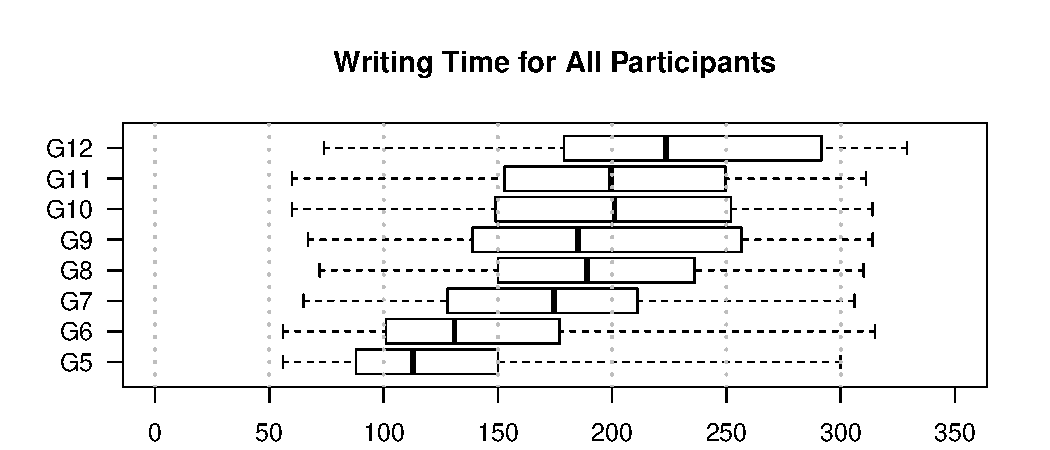
\includegraphics[width=\maxwidth]{figure/minimal-boxplots-minutes1-1} 

}



\end{knitrout}

\begin{knitrout}
\definecolor{shadecolor}{rgb}{0.969, 0.969, 0.969}\color{fgcolor}

{\centering 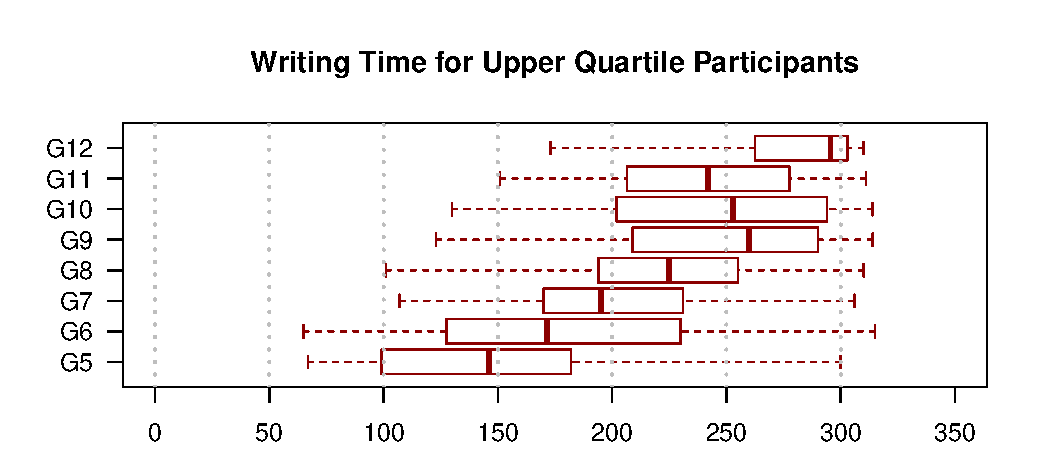
\includegraphics[width=\maxwidth]{figure/minimal-boxplots-minutes2-1} 

}



\end{knitrout}


\section{Dati par atsevišķajiem uzdevumiem}

\subsection{Vidējais vērtējums}

Ikviena uzdevuma vērtējums ir skaitlis no 0 līdz 10. Šajā tabulā apkopoti visu uzdevumu vidējie vērtējumi katrā no klašu grupām. Vidējo vērtējumu uzdevumam $X = \{ x_i \}$ aprēķina pēc formulas:

\[ E(X) = \frac{\sum_{i=1}^{n}{x_i}}{n}, \]

\noindent
kur $x_i$ ir $i$-tā skolēna vērtējums par uzdevumu $X$, bet $n$ ir visu attiecīgās klases darbu skaits: $n = \left| X \right|$.

% Vidējais rezultāts pa uzdevumiem
\begin{knitrout}
\definecolor{shadecolor}{rgb}{0.969, 0.969, 0.969}\color{fgcolor}
\begin{tabular}{l|l|l|l|l|l}
\hline
  & Uzd1 & Uzd2 & Uzd3 & Uzd4 & Uzd5\\
\hline
G5 & 3.98 & 3.97 & 5.07 & 2.27 & 2.58\\
\hline
G6 & 3.80 & 5.73 & 2.99 & 0.06 & 5.51\\
\hline
G7 & 7.59 & 5.99 & 7.14 & 1.54 & 5.69\\
\hline
G8 & 3.39 & 5.28 & 4.42 & 1.35 & 4.99\\
\hline
G9 & 4.04 & 4.59 & 3.05 & 3.42 & 5.24\\
\hline
G10 & 6.08 & 4.22 & 6.95 & 0.57 & 7.52\\
\hline
G11 & 7.00 & 2.74 & 3.47 & 0.46 & 2.12\\
\hline
G12 & 4.91 & 3.01 & 2.22 & 3.93 & 2.87\\
\hline
\end{tabular}


\end{knitrout}

\noindent
Viszemākais un visaugstākais vidējais vērtējums ir attiecīgi 11.\ klases 4.\ uzdevumam (1.75) un 12.\ klases 1.\ uzdevumam (7.09).

\begin{uzdevums}[11.4]
Doti 99 naturāli skaitļi. Zināms, ka nav tāda skaitļa, ar ko dalītos visi šie skaitļi, un ka jebkuru 50 skaitļu reizinājums dalās ar atlikušo 49 skaitļu reizinājumu. Pierādīt, ka visu 99 skaitļu reizinājums ir naturāla skaitļa kvadrāts.
\end{uzdevums}


\begin{uzdevums}[12.1]
Atrisināt nevienādību $9^x - 2 \cdot 3^x - 3 \leq 0$.
\end{uzdevums}






\subsection{Šenona entropija}

Entropiju uzdevuma $X$ vērtējumiem aprēķina pēc formulas:

\[ H(X) = - \sum_{i = 0}^{10}{p_i}\cdot \log_2{p_i}, \]

\noindent
kur $p_i = \frac{\left|\{ x \in X | x = i \}\right|}{\left| X \right|}$ ir varbūtība saņemt par uzdevumu $X$ vērtējumu $i$ (piemēram $p_0$ - vērtējumu "0 punkti" vai "uzdevums nav risināts" dalījums ar visu attiecīgās klases darbu skaitu). Ja kāds no vērtējumiem $i$ par attiecīgo uzdevumu nav sastopams, tad attiecīgo saskaitāmo entropijas formulā izlaiž.

Augsta entropija nozīmē augstu nenoteiktību. Ja visi vērtējumi par attiecīgo uzdevumu būtu vienādi, tad entropija ir 0. Ja visi vērtējumi no 0 līdz 11 ir vienādi bieži sastopami, tad entropija ir $\log2(11) \approx 3.46$. Pārāk zema entropija (piemēram tuvu 1 vai mazāka) nozīmē to, ka pats uzdevums vai tā vērtēšanas sistēma nav bijuši pārāk noderīgi olimpiādes dalībnieku punktu skaita diferencēšanai, jo pārāk daudzi vērtējumi ir vienādi.

\begin{knitrout}
\definecolor{shadecolor}{rgb}{0.969, 0.969, 0.969}\color{fgcolor}
\begin{tabular}{l|l|l|l|l|l}
\hline
  & Uzd1 & Uzd2 & Uzd3 & Uzd4 & Uzd5\\
\hline
G5 & 2.15 & 2.41 & 3.19 & 2.32 & 1.86\\
\hline
G6 & 2.53 & 3.31 & 2.01 & 0.30 & 3.31\\
\hline
G7 & 3.48 & 3.11 & 2.88 & 2.34 & 3.17\\
\hline
G8 & 1.66 & 2.81 & 1.33 & 1.55 & 3.05\\
\hline
G9 & 2.82 & 2.88 & 2.09 & 3.02 & 2.89\\
\hline
G10 & 2.57 & 2.53 & 2.86 & 0.63 & 3.13\\
\hline
G11 & 3.00 & 1.33 & 2.44 & 0.71 & 1.35\\
\hline
G12 & 2.72 & 1.84 & 1.96 & 2.84 & 1.76\\
\hline
\end{tabular}


\end{knitrout}


Viszemākā entropija ir bijusi 10.\ klases 5.\ uzdevuma vērtējumiem (0.80). Šie vērtējumi ir sekojoši (0 punkti - 252 darbos; 1 punkts - 10 darbos, 2 punkti - 4 darbos, 3 punkti - 1 darbā, 5 punkti - 1 darbā, 10 punkti - 4 darbos).

\begin{uzdevums}[10.5]
Uz taisnstūra $ABCD$ diagonāles $BD$ iespējams atrast iekšēju punktu $P$ tā, ka
$\angle PAB = \angle PCB$. Pierādīt, ka $ABCD$ ir kvadrāts!
\end{uzdevums}






\subsection{Uzdevuma korelācija ar pārējo vērtējumu summu}

Izvēļu testu ({\em multiple choice exams}) analīzē bieži izmanto {\em biseriālo korelācijas koeficientu} --- kāda ir korelācija starp eksāmena kopīgo rezultātu un atbildēm (pareizas/nepareizas) uz konkrēto uzdevuma jautājumu. Ar šo skaitlisko kritēriju var atrast tos testu jautājumus, kuri varētu būt mulsinoši formulēti vai arī nemēra tās pašas prasmes, ko citi šī paša testa uzdevumi.

Protams, olimpiāde nav izvēļu tests (un par katru no jautājumiem ir vairāk vērtējumu nekā tikai 0 vai 1). Tomēr arī šajā gadījumā korelācija var noderēt. Ja uzskatām, ka olimpiāde kopumā mēra noteikta veida matemātiskas prasmes, tad par katru uzdevumu var uzdot jautājumu: Cik labi šis uzdevums palīdz mērīt to pašu, ko olimpiādes uzdevumu komplekts kopumā? Ja konkrētais uzdevums labi ``iederas'' starp citiem, tad korelācija būs augsta, ja tas mēra kādas stipri atšķirīgas prasmes nekā citi tās pašas klases uzdevumi, tad korelācija būs mazāka. Korelāciju rēķina pēc šādas formulas:

\[ \mbox{cor}(X,Y) = \frac{\sum_{i=1}^{n}{x_i y_i} - n \cdot E(X) \cdot E(Y)}{\sqrt{\sum_{i=1}^{n}{x_i^2} - n \cdot E(X)^2}
\cdot \sqrt{\sum_{i=1}^{n}{y_i^2} - n \cdot E(Y)^2}}, \]

\noindent
kur $x_i$ ir $i$-tā dalībnieka vērtējums par uzdevumu $X$, $y_i$ ir vērtējumu summa par visiem 4 atlikušajiem uzdevumiem, $n$ --- darbu skaits attiecīgajā klasē, $E(X)$ apzīmē $x_i$ aritmētisko vidējo.

Korelācijas koeficients vienmēr ir intervālā $[-1,1]$. Teorētiski varētu gadīties arī negatīva korelācija, t.i. tāds uzdevums, kuru veiksmīgākie olimpiādes dalībnieki risināja sliktāk nekā mazāk veiksmīgie. Tad paša uzdevuma vai vērtēšanas sistēmas korektums radītu nopietnas šaubas. Olimpiāžu praksē tomēr negatīvas korelācijas nav vērojamas. Salīdzinoši zemas uzdevuma vērtējuma korelācijas ar citiem uzdevumiem ļauj atrast tos uzdevumus, kuru tēma vai vērtēšanas kritēriji ir būtiski atšķīrušies no citiem uzdevumiem tajā pašā klases 5 uzdevumu komplektā.

\begin{knitrout}
\definecolor{shadecolor}{rgb}{0.969, 0.969, 0.969}\color{fgcolor}
\begin{tabular}{l|l|l|l|l|l}
\hline
  & Uzd1 & Uzd2 & Uzd3 & Uzd4 & Uzd5\\
\hline
G5 & 0.18 & 0.21 & 0.37 & 0.38 & 0.23\\
\hline
G6 & 0.15 & 0.07 & 0.07 & 0.12 & 0.15\\
\hline
G7 & 0.27 & 0.22 & 0.43 & 0.29 & 0.28\\
\hline
G8 & 0.24 & 0.06 & 0.10 & 0.06 & 0.12\\
\hline
G9 & 0.33 & 0.28 & 0.29 & 0.33 & 0.38\\
\hline
G10 & 0.01 & 0.05 & 0.12 & -0.01 & 0.02\\
\hline
G11 & 0.11 & 0.22 & 0.24 & 0.24 & 0.36\\
\hline
G12 & 0.07 & 0.28 & 0.26 & 0.37 & 0.41\\
\hline
\end{tabular}


\end{knitrout}

Mazākās korelācijas ar citiem tās pašas klases uzdevumiem ir 10.\ klases 2.\ uzdevumam (0.13) un 12.\ klases 4.\ uzdevumam (0.05). Šos uzdevumus varētu uzskatīt par ``visjocīgākajiem'', kas prasīja prasmes, kas stipri atšķiras no citos uzdevumos nepieciešamajām.

\begin{uzdevums}[10.2]
Dotas divas paralēlas taisnes. Uz vienas no tām atzīmēti 14 zaļi punkti, uz otras -- 14 sarkani punkti. Kādu lielāko skaitu nogriežņu, kuriem viens galapunkts ir zaļš, bet otrs -- sarkans, var novilkt tā, lai tie nekrustotos? Saka, ka nogriežņi krustojas, ja tiem ir kopīgs iekšējais punkts, t.i., ja tiem ir kopīgs tikai galapunkts, tie nekrustojas.
\end{uzdevums}


\begin{uzdevums}[12.4]
Vai kvadrātu ar malas garumu 10 var noklāt ar 25 ``krustiņiem'' (skat. zīm.), kuri sastāv no 5 kvadrātiem ar malas garumu 1? ``Krustiņi'' drīkst pārklāties, kā arī iziet ārpus dotā kvadrāta malām.\\

\includegraphics[width=14mm]{pentomino-x.png}
\end{uzdevums}







\subsection{Vērtējumu atšķirības zēniem un meitenēm}

Vērtējumu atšķirību konkrētas klases uzdevumam $X$ aprēķina kā divu vidējo vērtību starpību:

\[ \Delta_{\mbox{gender}}(X) = E\left(X_{\mbox{male}}\right) - E\left(X_{\mbox{female}}\right), \]

\noindent
kur $X_{\mbox{male}}$ ir visi attiecīgās klases zēnu vērtējumi un  $X_{\mbox{female}}$ ir attiecīgās klases meiteņu vērtējumi, un $E(X)$ - skaitļu virknes $X$ aritmētiskais vidējais.

\begin{knitrout}
\definecolor{shadecolor}{rgb}{0.969, 0.969, 0.969}\color{fgcolor}
\begin{tabular}{l|l|l|l|l|l}
\hline
  & Uzd1 & Uzd2 & Uzd3 & Uzd4 & Uzd5\\
\hline
G5 & 0.05 & -0.06 & -0.08 & 0.19 & 0.02\\
\hline
G6 & 0.03 & -0.02 & -0.15 & 0.01 & -0.22\\
\hline
G7 & 0.38 & -0.05 & 0.32 & -0.24 & 0.27\\
\hline
G8 & 0.36 & -0.57 & -0.10 & 0.77 & 0.26\\
\hline
G9 & 0.23 & 0.72 & 0.11 & 0.38 & -0.06\\
\hline
G10 & 1.00 & 0.15 & -0.23 & 0.67 & 0.23\\
\hline
G11 & 1.02 & 0.04 & 0.62 & 0.04 & 0.22\\
\hline
G12 & 0.44 & -0.12 & 0.01 & 0.70 & 0.21\\
\hline
\end{tabular}


\end{knitrout}

Katram no uzdevumiem atrasta zēnu un meiteņu vidējo vērtējumu starpība. Pozitīvs skaitlis nozīmē to, ka zēnu vērtējums bija augstāks, negatīvs skaitlis --- to, ka meiteņu vērtējums bija augstāks. Vislielākās priekšrocības zēniem bija risinot 6.\ klases 5.\ uzdevumu (1.88 punktu pārsvars); savukārt meitenēm --- risinot 5.\ klases 4.\ uzdevumu (0.63 punktu pārsvars). Neparasti, ka abi šie uzdevumi ir par līdzīgu tēmu --- rūtiņu laukuma aizpildīšanu ar figūriņām. Šī pārskata mērķis nav noskaidrot, vai atšķirības ir statistiski būtiskas. Varbūt dzimumu atšķirības radīja ne vien pats uzdevums, bet arī noteikta veida vērtēšanas kritēriji. Diez vai to ir iespējams precīzi noskaidrot, ja pēc olimpiādes darbu labošanas pagājis vairāk nekā 1 gads.

\begin{uzdevums}[6.5]
Rūtiņu kvadrātā $5 \times 5$ iekrāsot iespējami maz rūtiņu tā, lai atlikušajā daļā vairs nevarētu ievietot nevienu zīmējumā redzamo figūru (tā var būt gan pagriezta, gan apgāzta). Pamatot, ka iekrāsoto rūtiņu skaits ir mazākais iespējamais!\\
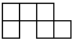
\includegraphics[width=20mm]{hexomino.png}
\end{uzdevums}


\begin{uzdevums}[5.4]
Kvadrāts sastāv no $8 \times 8$ vienādām kvadrātiskām rūtiņām. Tas sagriezts daļās tā, ka griezumi iet pa rūtiņu robežām. Kāds lielākais skaits daļu var būt tādas kā zīmējumā attēlotā figūra (figūras var būt pagrieztas jebkurā stāvoklī)?\\
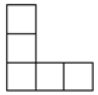
\includegraphics[width=14mm]{pentomino-v.png}
\end{uzdevums}



\end{document}
